% ==============================================================================    
\chapter{Pixel readout ASICs and assembly calibration}
\label{ch:FE_electronics}
% ==============================================================================    

% ----------------------------- %
\tikzstyle{block} = [rectangle, draw, text width=5em, text centered, rounded corners, minimum
height=4em]
\usetikzlibrary{backgrounds,fit,decorations.pathreplacing} 
% ----------------------------- %

One of the key components of the detector systems is the readout
electronics. Each experiment, depending on the requirements, has its
own specific electronics. 


% But the basic principles of the electronics
% and optimisations of the signal-to-noise ratio remain similar for
% different applications.

In this chapter, we will review the basic principles and requirements
of the Timepix3 hybrid pixel readout chip which is used as a test
vehicle to study thin and active-edge sensors as described in the
following chapters. The calibration method for the Timepix3 assemblies
and also the noise measurements are explored in this chapter.

%\section{Generic pixel chip properties}
\section{The Timepix3 hybrid readout ASICs}
\label{sec:TimepixChip}

The hybrid readout chip acquires the short ionisation current pulses
generated in the sensor by the passing of a charged particle. For
acquiring this short pulse, the time response of the readout must be
tailored to optimise the minimum detectable signal, the measurement of
energy deposition in the detector, the event rate capability, timing
measurement of the signal and the insensitivity of the system to the
pulse shape. Finally, the signal is digitised and stored. Robustness
to radiation and low power consumption are other important
considerations to be addressed amongst others.


The Timepix~\cite{art:tmpx,Timepix3Poikela} hybrid pixel detector
readout chip family, designed by the Medipix
collaboration~\cite{medipixCollaboration}, is a general purpose
front-end electronics and can measure precisely the energy deposited
in the sensor and also provides accurate timing information. These
chips are used in a wide range of applications such as high energy
physics and medical imaging. The Timepix3 ASIC is deployed for the
CLIC vertex detector R\&D to study the feasibility of thin sensors and
also active-edge sensors as described in the coming chapters.

\cref{fig:detectorFunctions} schematically shows the basic signal flow
in a Timepix3-like hybrid pixel detector. Both analogue and digital
circuitry are combined for signal processing.

The incident radiation deposits energy in the sensor which is
converted to an electrical signal. A high rate of particles can be
handled in a semiconductor detector because the sensor pulse is very
short (few nanoseconds). A charge sensitive preamplifier is needed to
amplify the short signal pulse. As seen in \cref{sec:chargeInSi}, the
amount of signal charge is small and subject to statistical
fluctuations. The preamplifier should be designed in a way to minimise
the electronics noise (see \cref{sec:noise} for a discussion of the
noise sources). The sensor capacitance and the input capacitance of
the amplifier play a critical role in the optimisation of the
signal-to-noise ratio (SNR): the lower the capacitance, the higher the
SNR.

The preamplifier is implemented in a Krummenacher
topology~\cite{KRUMMENACHER1991527}, where the return to the baseline
of the amplified signal is done with a tunable current
(I\textsubscript{krum}). The higher I\textsubscript{krum}, the faster
the return and the shorter the pulse. For the Timepix readout chip
family, a pulse shaper is embedded in the preamplifier which outputs a
triangular-like pulse shape where the rising edge is imposed by the
time response of the preamplifier and the slope of the falling edge
dictated by the I\textsubscript{krum} current.

% After the preamplifier, the pulse shaper is responsible for the
% improvement of the SNR. It modifies the frequency response of the
% signal to improve the signal and attenuate the noise. Since this
% operation reduces the bandwidth of the signal, the duration of the
% pulse will increase. As a detector must cope with a high rate of
% pulses, the width of the pulse must be optimised to reduce the
% pile-up. The analogue processing chain of the Timepix readout chip
% family does not include an explicit pulse shaper. The pulse shaping is
% embedded in the preamplifier, which outputs a triangular-like pulse
% shape where the rising edge is imposed by the time response of the
% preamplifier and the falling edge dictated by the
% I\textsubscript{krum} current.

A discriminator is used to compare the signal level to a tunable
threshold voltage and to discriminate signal from background
noise. Both polarities (electrons and holes) are accepted by the front
end.

When the pulse height passes the threshold in the discriminator,
counters in the digital part of the readout chip are incremented to
measure the energy and the arrival time of the signal.

\begin{figure}[htbp]
  \centering
  \begin{tikzpicture}[node distance = 2.5cm, auto]
    \begin{scope}[x={(image.south east)},y={(image.north west)}]

      \coordinate (input);
      \node [block, right of=input] (sens) {Sensor};
      \node [block, right of=sens] (preamp) {Preamplifier/ Shaper};
      %% \node [block, right of=preamp] (pulse) {Pulse shaping};
      \node [block, right of=preamp] (discr) {Discriminator};
      \node [block, right of=discr] (conv) {TOT/TOA counters};
      \coordinate[right of=conv] (output);

      \draw[arrows=->] (input) -- node [text
      width=2cm,midway] {Incident radiation} (sens);
      \draw[arrows=->] (sens) -- (preamp);
      \draw[arrows=->] (preamp) -- (discr);
      %\draw[arrows=->] (pulse) -- (discr);
      \draw[arrows=->] (discr) -- (conv);
      \draw[arrows=->] (conv) -- node [text width=1.5cm,midway]
      {Digital data bus} (output);

      % \draw[] (sens) -- (discr.south);
      \draw[decorate,decoration={brace, mirror}, thick] (sens.south) to
      node[below,below] (bracket) {Analogue domain}
      (discr.south);

      \draw[decorate,decoration={brace, mirror}, thick] (conv.south
      west) to node[below,below] (bracket) {Digital domain} (conv.south
      east);

      \draw[decorate,decoration={brace}, thick] (preamp.north) to
      node[above, above] (bracket) {Readout chip} (conv.north);

    \end{scope}
  \end{tikzpicture}
  \caption{Schematic overview of basic signal flow in a Timepix-like
    hybrid pixel detector. The energy deposited in the sensor by the
    incident radiation is converted to an electrical signal. The
    signal is integrated in the preamplifier, shaped by the pulse
    shaper and compared to a programmable threshold by the
    discriminator. The digital part of the readout chip digitises the
    signal for storage and analysis using counters for timing and
    energy measurements.}
  \label{fig:detectorFunctions}
\end{figure}


An overview of the main parameters of the Timepix3 readout chip is
given in~\cref{tab:timepixOverview}. It consists of a $256\times256$
pixel matrix with a pitch of $55\,\micron$. This chip allows for three
operation modes: photon counting (PC), Time-over-threshold (TOT) and
Time-of-Arrival (TOA) measurements. In addition, Timepix3 allows for
simultaneous measurement of the TOT and the TOA. In the photon
counting mode, a counter is incremented each time a photon hits the
pixel and deposits an energy higher than the programmable threshold.



\begin{table}[htbp]
  \centering
  \caption{Overview of the main parameters of the Timepix3 readout ASIC.}
  \label{tab:timepixOverview}
  \begin{tabular}{l l}
    \toprule
    Pixel Matrix& $256\times256$\\
    Pixel Pitch & $55\,\micron$\\
    Technology & 130~nm CMOS\\
    Measurement Modes & 10 bit TOT and 18 bit TOA \\
                & 18 bit TOA only \\
                & 10 bit PC and 14 bit integral TOT \\
    Clock speed & Up to $40\,\megahertz$ for TOT and general TOA \\
                & $640\,\megahertz$ for FTOA \\
    Readout Type & Data driven or Frame based \\
    Electronic Noise (without sensor) & $<70$ e\textsuperscript{-} RMS\\
    \bottomrule
  \end{tabular}
\end{table}


\cref{fig:TOT_TOA_concept} schematically shows the energy and the
timing measurements of the signal. The Time-over-threshold (TOT)
allows for the measurement of the energy deposited in a pixel. The
time above the programmable threshold of the triangular-like signal
pulse is proportional to the energy deposited and during this time,
the TOT counter is incremented.

The Time-of-Arrival (TOA) measures the arrival time of a hit and is
used for a time stamping of the hits. A general TOA counter runs with
the general $40\,\megahertz$ clock. When the amplifier output exceeds
the pixel threshold, the discriminator output rises and the fast TOA
(FTOA) $640\,\megahertz$ counter runs until the rising edge of the
general clock. A combination of the global TOA counter and the FTOA
counters is used to calculate the arrival time of the hits (or the
pixel TOA). The FTOA counter is also used to increase the precision of
the TOT measurement.

\begin{figure}[htbp]
  \centering 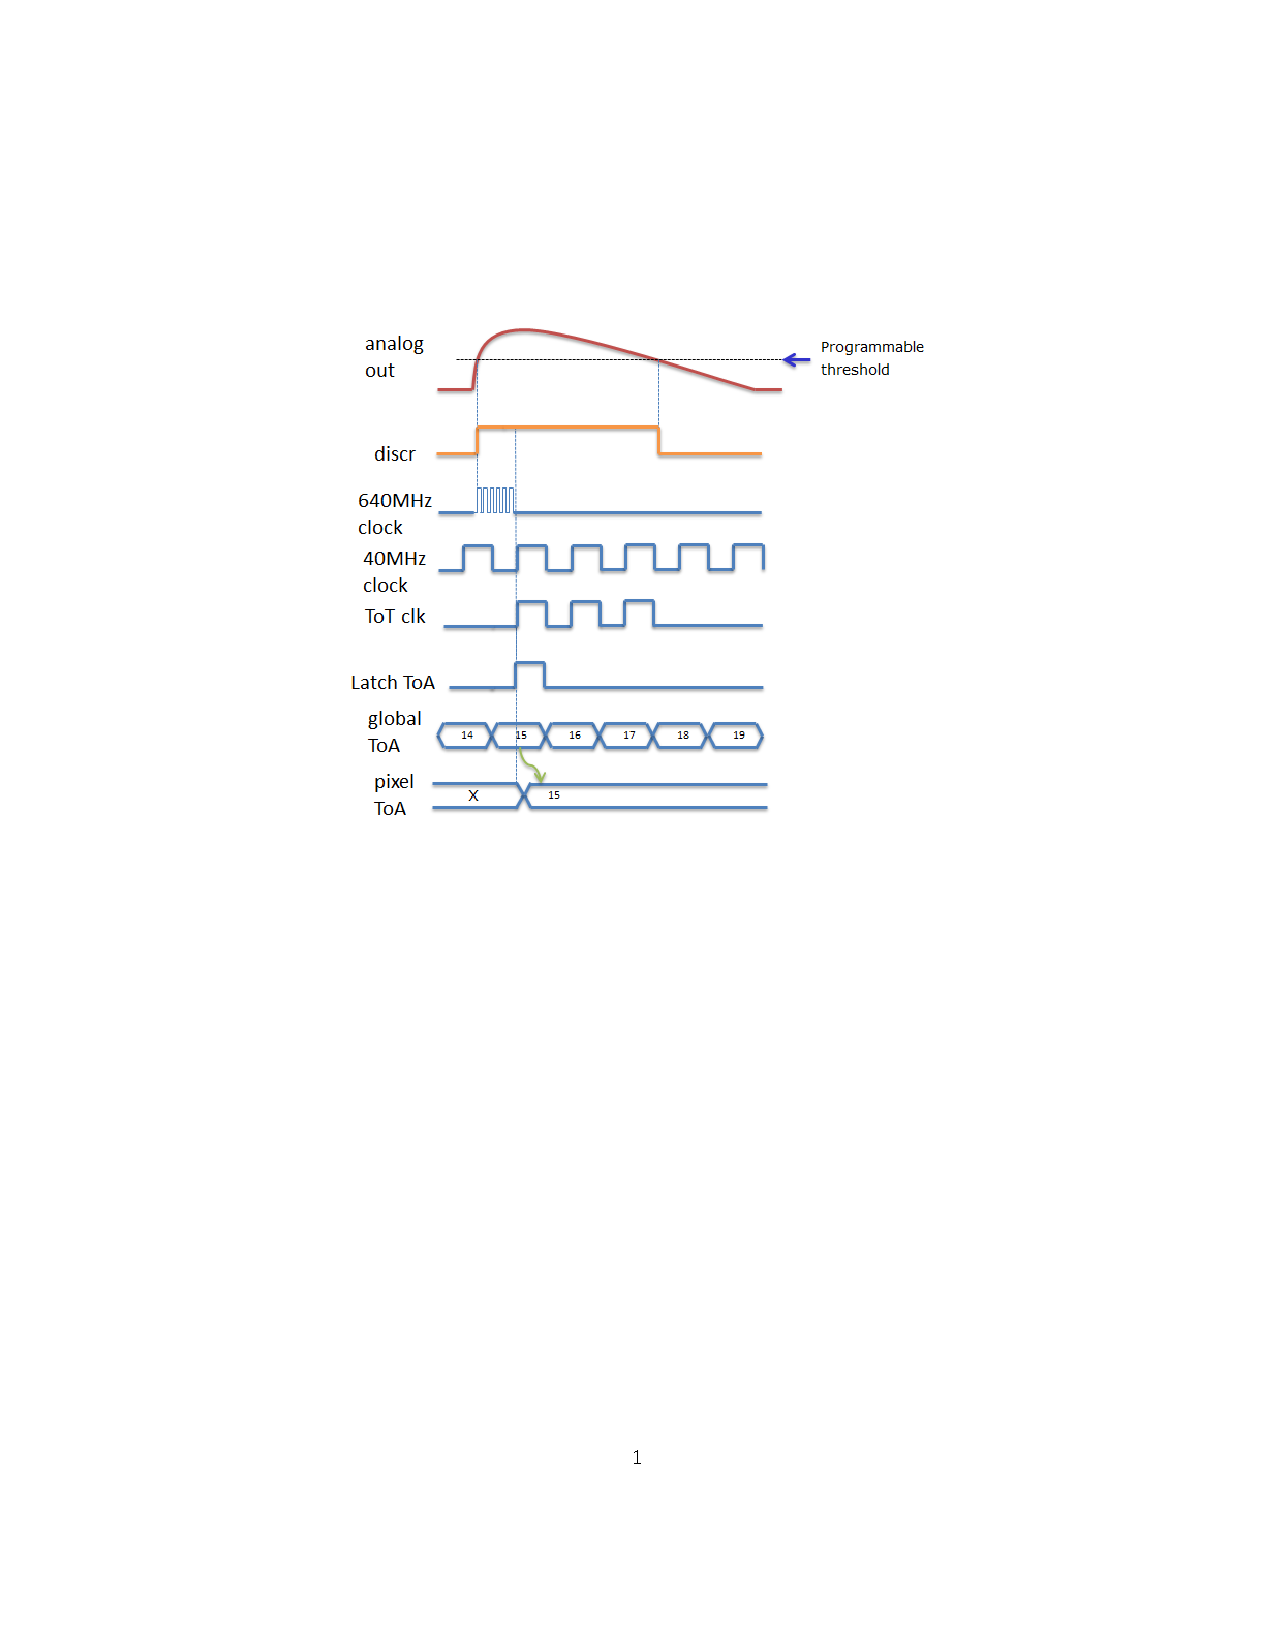
\includegraphics[width=0.7\textwidth, trim = 50mm 140mm
    60mm 50mm, clip]{figures/Calibration/TOT_TOA_explanation.pdf}
  \caption{Schematic overview of the Time-over-Threshold (TOT) and
    Time-of-Arrival (TOA) measurements for the Timepix3 readout
    chips. From~\cite{Timepix3Poikela}.}
  \label{fig:TOT_TOA_concept}
\end{figure}

The Timepix3 readout chip allows for a data-driven zero-suppressed
readout mode which can reach higher readout rates than the frame based
mode. In the data driven mode, after a hit is processed by the pixel,
a data packet containing the TOT and the TOA information is
immediately sent off the chip. This reduces significantly the dead
time of the pixels hit while the other pixels stay active and allows
to reach very high readout rates of up to
40~Mhits/(s~$\cdot$~\cmsquared).

The different settings of the chip are controlled using programmable
DACs such as the I\textsubscript{krum}, threshold, polarity of the
sensor and the clock speed.



\subsection{SPIDR readout system for Timepix3}
\label{sec:TimepixReadout}

The SPIDR (Speedy PIxel Detector Readout) readout
system~\cite{Visser:2015bsa} is used for the Timepix3 data
acquisition. This system is able to handle high rates of data sent by
the Timepix3 ASIC at full speed. This is achieved with Xilinx Virtex-7
FPGA~\cite{XilinxVirtex7} and a 10~Gb Ethernet link.

\cref{fig:Timepix3board_SPIDR} shows the Timepix3 chip and the SPIDR
readout board. Voltage regulators on the Timepix3 chip board, allow to
set the voltage of the programmable DACs.

\begin{figure}[htbp] \centering
  \begin{subfigure}[b]{0.3\textwidth}
    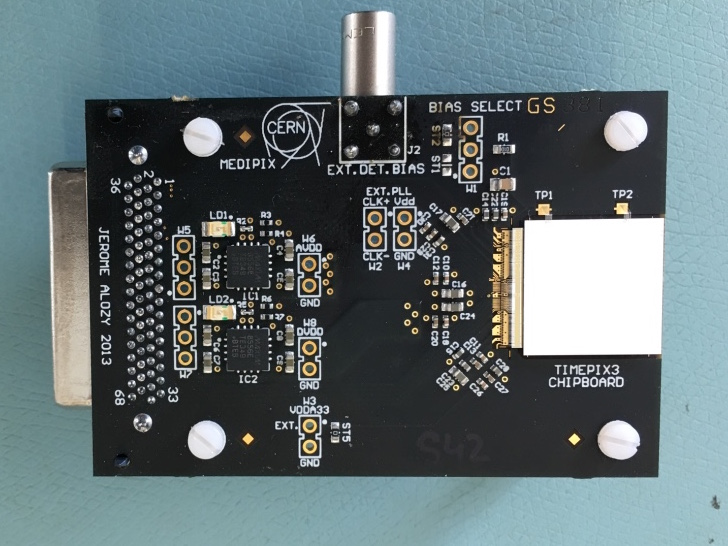
\includegraphics[width=\textwidth]{./figures/Calibration/Timepix3board2.jpg}
    \caption{}\label{fig:Timepix3board_PCB}
  \end{subfigure}\hfill
  \begin{subfigure}[b]{0.65\textwidth}
    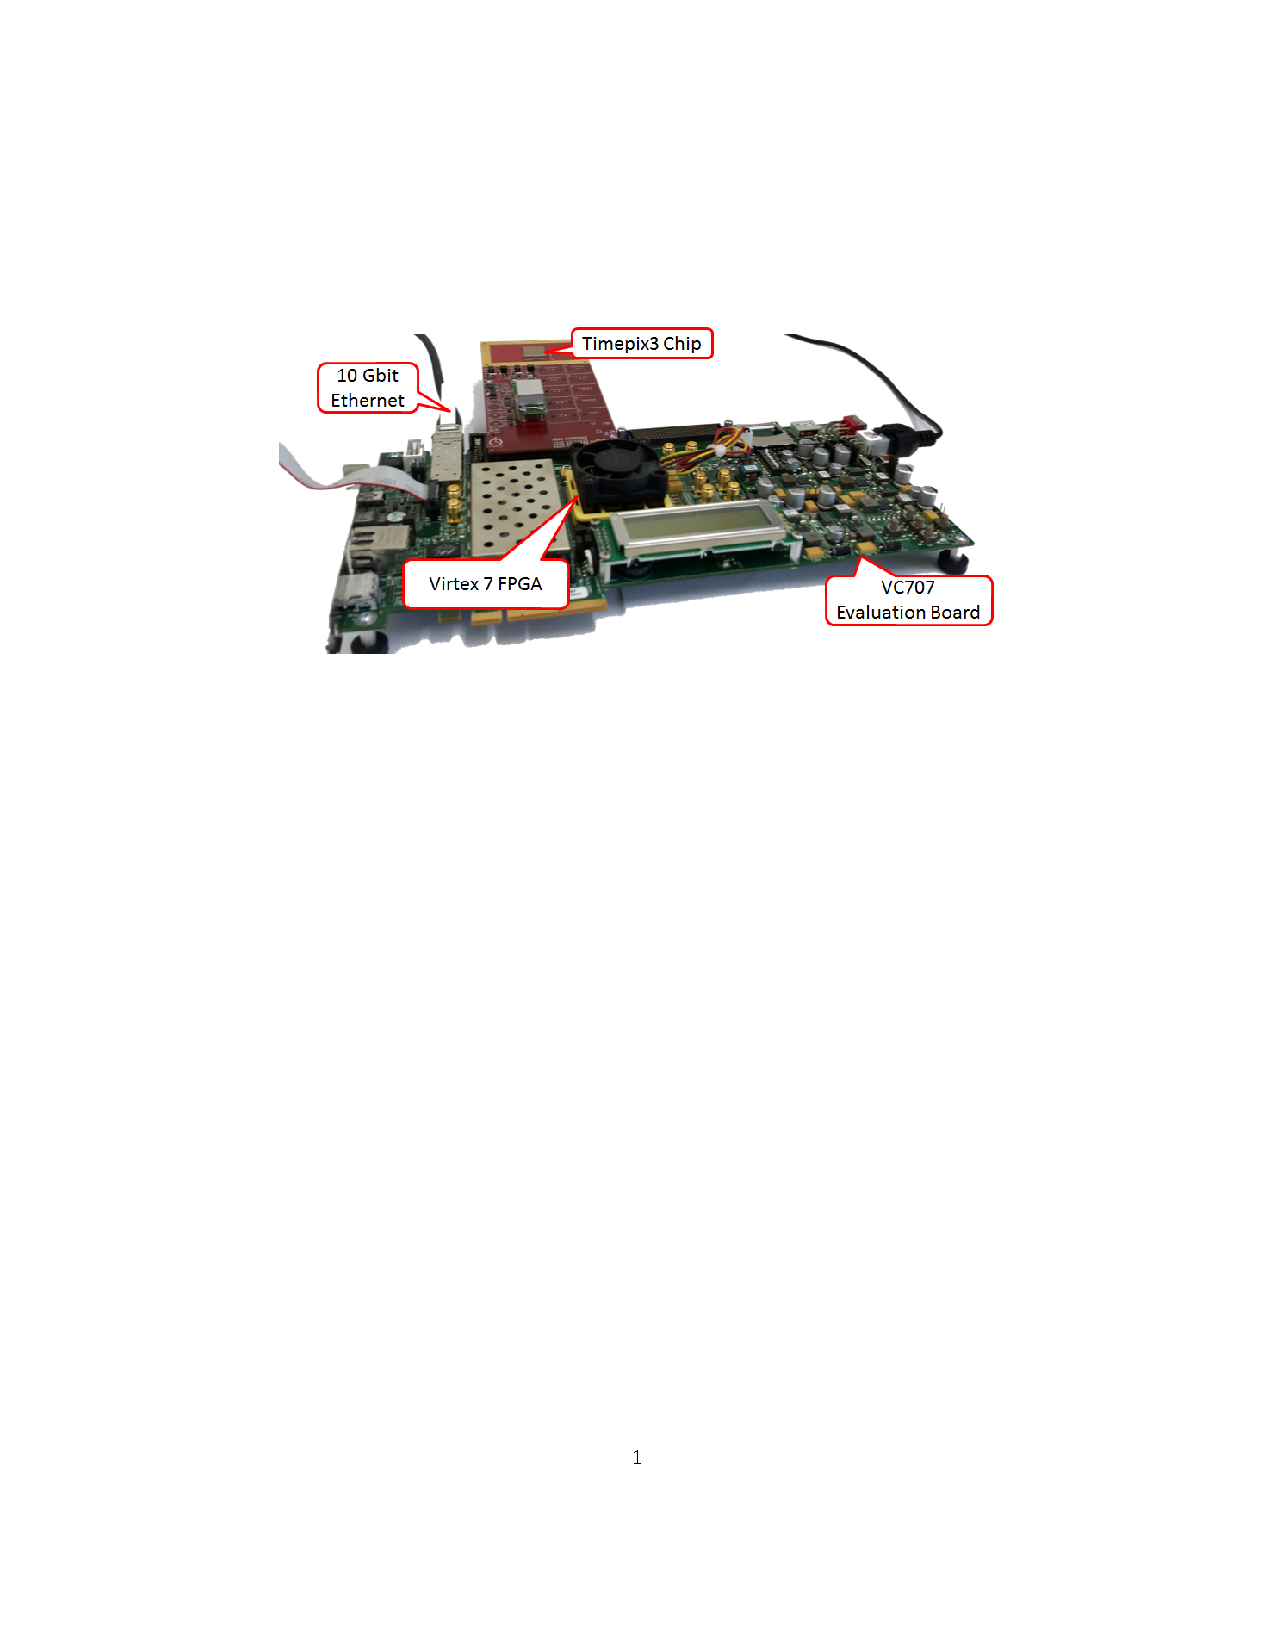
\includegraphics[width=\textwidth, trim = 50mm 170mm 40mm 50mm,
      clip]{./figures/Calibration/SPIDRboard.pdf}
    \caption{}
  \end{subfigure}
  \caption{(a) Timepix3 chip board and (b) SPIDR readout board
    from~\cite{Timepix3Poikela}.}
  \label{fig:Timepix3board_SPIDR}
\end{figure}


%% --------------------------------------------- %%
\section{Timepix3 assemblies}\label{sec:Timepix3Assemblies}
A summary of the Timepix3 assemblies used in this study is shown in
\cref{tab:Timepix3Assemblies}. Advacam sensors~\cite{AdvacamRef} of
thickness $50$-$150\,\micron$ are bump-bonded to Timepix3 readout
chips.

\begin{table}[htbp]
  \centering
  \caption{Details of different Advacam planar pixel sensors
    bump-bonded to Timepix3 readout ASICs and studied in calibration
    and test beams. For active-edge sensors, the edge distance is
    defined by the distance between the last pixel implant and the
    physical sensor edge (see \cref{ch:ActiveEdgeSensors}).}
  \label{tab:Timepix3Assemblies}
  \resizebox{\textwidth}{!}{\begin{tabular}{lccccc}
    \toprule
    Timepix3 ID & Thickness [\micron] & Type & Edge distance [\micron] & Guard-ring potential & Assembly\\
    \midrule
     W19\_G7 & 50 & n-in-p & 20 & Without GR & 20-NGR-50 \\
     W19\_F7 & 50 & n-in-p & 23 & Floating & 23-FGR-50 \\
     W19\_L8 & 50 & n-in-p & 28 & Grounded & 28-GNDGR-50 \\
     W19\_C7 & 50 & n-in-p & 55 & Grounded & 55-GNDGR-50 \\ \hline
     W5\_E2 & 100 & n-in-p & 55 & Grounded & 55-GNDGR-100 \\ \hline
     W5\_F1 & 150 & n-in-p & 55 & Grounded & 55-GNDGR-150 \\ %% \hline
     %% W2\_J5 & 300 & p-in-n & - & - & - \\
    \bottomrule
  \end{tabular}}
\end{table}

%% --------------------------------------------- %%
\section{Electronic noise}
\label{sec:noise}

Electronic noise places a limit on the minimum detectable signal
level. It defines the ability to distinguish signal levels and their
precision of measurement. Thermal excitations and sensor leakage
currents are important sources for the noise. The electronic noise can
be measured as explained further in
\cref{sec:thresholdCalibration}. For Timepix3 readout chips, the
electronic noise before bonding to any sensor is less than
70~e\textsuperscript{-} RMS and after bonding it increases to
$\sim80$~e\textsuperscript{-} RMS due to the capacitance of the sensor
and its leakage current.

%% --------------------------------------------- %%
\section{Threshold dispersion and equalisation} 
\label{sec:ThresholdEqualisation}


In semiconductor electronics, manufacturing imperfections cause
variations in the performance of the devices within the same chip. In
this regard, the programmable global threshold of the chip is one of
the most affected parameters. 

A global threshold voltage generated by a programmable DAC
(Digital-to-Analogue Converter) in the periphery of the chip is
applied to the all the pixel discriminators. But the effective
threshold of each discriminator varies from one pixel to another. To
overcome this dispersion, a 4-bit local threshold adjustment is
applied to each pixel in order to achieve a uniform global
threshold. The photon counting mode is used in the procedure. The
equalisation consists of adjusting this local threshold as shown in
\cref{fig:THLequalisation} for the assembly W19\_L8.

First, the local threshold is set to its minimum value
(mask~0000). For each pixel, the global threshold DAC (THL) is scanned
from a level of no counts (threshold above the chip noise) to a level
where all the pixels count (threshold close to the noise level). This
results in an S-shaped curve (an example is shown later in
\cref{fig:scurve_example}). The middle of this curve, where the
curvature changes, corresponds to the mean value of the noise. The
mean value of the noise is measured for all pixels and filled into the
histogram for mask~0000 as shown in \cref{fig:THLequalisation}. The
same measurement is then repeated by setting the adjustment bits to
their maximum value (mask~1111) and THL is scanned again. 

For each pixel, the operation range is thus known. Assuming a linear
relationship between the two points, the adjustment threshold is set
in such a way that the global threshold will remain uniform across the
matrix. After equalisation the response of the chip becomes more
uniform even though some dispersion remains ($\sim40$ electrons).

%% \cref{fig:THLequalisation} shows the threshold equalisation for the
%% assembly W19\_L8. After equalisation the response of the chip becomes
%% more uniform even though some dispersion remains.

\begin{figure}[htbp] 
  \centering
  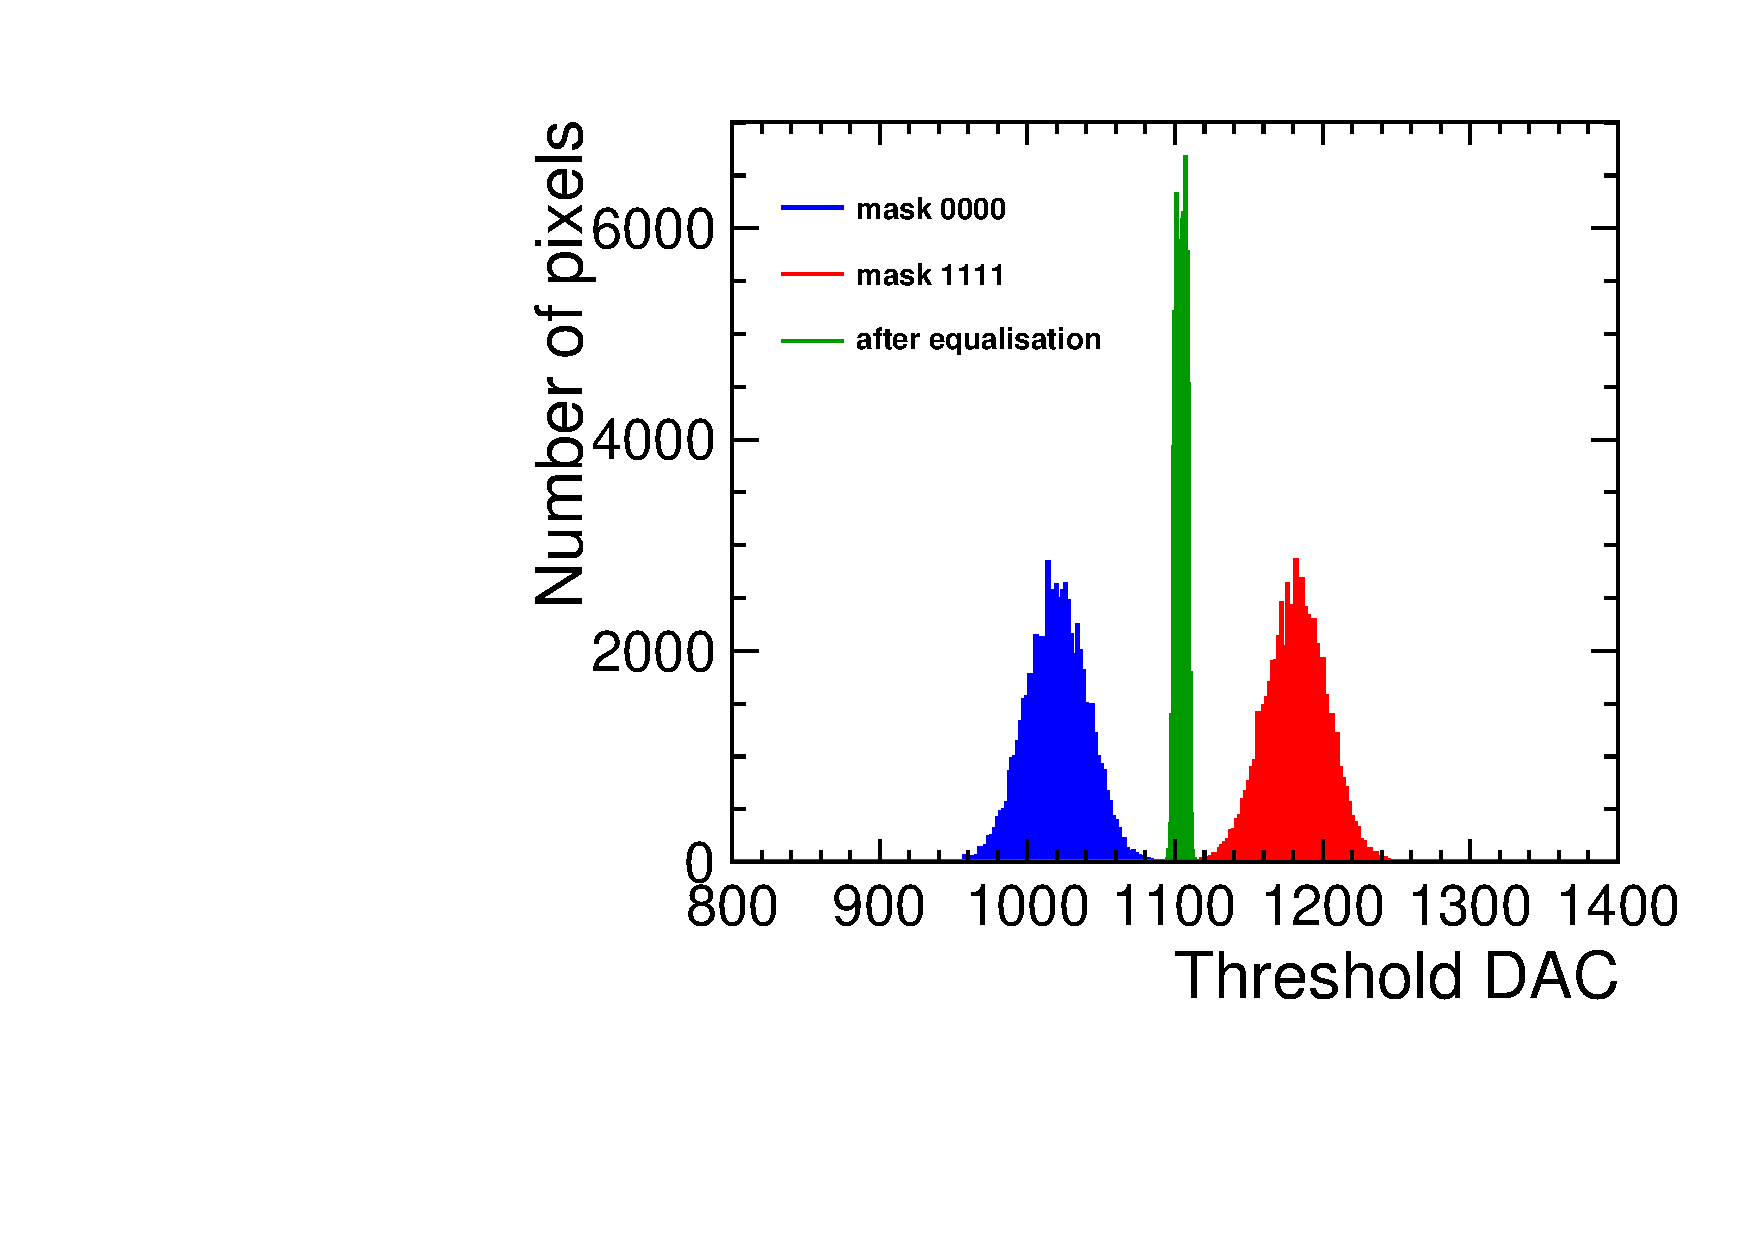
\includegraphics[width=0.6\textwidth]{./figures/Calibration/THLequalisation_W19_L8.pdf}
  \caption{Spread of pixel responses for the assembly W19\_L8 during
    equalisation for the local threshold set at its minimum value
    (mask 0000), to its maximum value (mask 1111) and after
    equalisation.}
  \label{fig:THLequalisation}
\end{figure}


%% --------------------------------------------- %%
\section{Operating threshold} 
\label{sec:operatingThreshold}

The electronic noise and the threshold dispersion are important
parameters to determine the operating threshold of the readout
ASIC. The operating threshold for the Timepix3 chip is set to 6 times
the electronic noise RMS added in quadrature to the threshold
dispersion. This threshold significantly reduces the detection of
noisy hits. The very low noise of the Timepix3 chip allows for
operating the chip at a low threshold of approximately 500 electrons
and thereby the detection of small signals. Sometimes, at this
threshold a few pixels show a high rate of hits in absence of incident
radiation (hot pixels) and they are manually masked to be able to
operate the chip at the lowest possible threshold.

The operating threshold affects significantly the spatial resolution
of the device. A lower threshold allows for a higher detection of the
charge sharing. For this reason, it is important to minimise the
electronic noise and the threshold dispersion.


%%%%%%%%%%%%%%%%%%%%%%%%%%%%%%%%%%%%%%%%%%%%%%%%%%
\section{Calibration} 
\label{sec:calibration} 

The aim of the calibration is to parametrise the measurements done by
the readout chip, namely the relationship between the threshold DAC
and the TOT with the energy deposited in the sensor as well as the
relation between the TOA measurement and the time of arrival of the
particle (in seconds). The unit to describe the energy deposited in
the sensor can be in $\kev$ or the number of electron-hole pairs
produced knowing that the average energy required to produce an
electron-hole pair is $\sim3.6\,\ev$ (see \cref{sec:silicon}).

In this work we focus on the threshold DAC and the TOT calibration and
the unit to describe the energy deposition is chosen to be the number
of electron-hole pairs generated (or to simplify in number of
electrons).

The threshold DAC and TOT calibration can be achieved using two
methods. The first one consists of the use of photons from radioactive
sources with a characteristic decay energy or photons from X-ray
fluorescence (XRF) with a characteristic emission
energy~\cite{AlipourTehrani:2054922}. The photon being stopped in the
sensor, it deposits its full energy. Since the energy of the photon is
known, its relation to the threshold DAC or TOT can be characterised.

The second method consists of the use of an internal analogue test
pulse generator. The Timepix3 readout ASICs provide an internal test
pulse generator which can be used for calibration. In each pixel, a
capacitor allows for injecting a charge by applying a voltage step
over it. The injected charge is given by:

\begin{equation}
  Q = C \cdot \Delta V \; ,
  \label{eq:testpulseCharge}
\end{equation}

where Q is the injected charge, C the injection capacitance and
$\Delta V$ the voltage difference applied. The injection capacitance
can vary from pixel to pixel and also from chip to chip. From chip
design simulations, the metal-to-metal capacitance can be
extracted. For the Timepix3 readout chip a capacitance of
$20.2$~e\textsuperscript{-}/mV (or about 3.2~fF) is expected. This
value has also been cross-checked with X-ray sources and the expected
value has been validated~\cite{MedipixCapa}.

For calibration with the chip bump-bonded to a sensor, the sensor is
biased to full depletion to reduce the capacitive noise.



%% --------------------------------------------- %%
\subsection{Threshold-energy calibration} 
\label{sec:thresholdCalibration}

\cref{sec:operatingThreshold} describes the selection of the operating
threshold DAC (Digital-to-Analogue Converter) for a Timepix3 readout
chip. This threshold can be translated into an effective energy. The
counting mode is used for this measurement.

For Timepix3 assemblies, the threshold is calibrated using test pulses
at four different heights corresponding to 0, 1000, 3000 and 6000
electrons. For each pulse height, 200 pulses are sent to the pixels in
the diagonal of the matrix and the threshold DAC is scanned with a
step size of 2 from a level of no counts (threshold above the signal)
to a level where all the pixels count (threshold close to the noise
level) resulting in an S-shaped curve as shown in
\cref{fig:scurve_example}. The readout electronics noise smears the
ideal sharp turn on and generates the S-curve. At the maximum gradient
of the S-curve, the threshold DAC corresponds to the pulse
amplitude. The S-curve is fitted with a sigmoid function defined as:

\begin{equation}
f(x)= {1 \over {1+e^{-x}}} \; .
\end{equation}

The derivative of the S-curve or the sigmoid function is a Gaussian as
shown in \cref{fig:deriv_example} with a mean at the maximum gradient
of the S-curve.

% The derivative at each point of the S-curve corresponds to
% the slope of the line connecting it to its neighbour.

\begin{figure}[htbp] \centering
  \begin{subfigure}[b]{0.45\textwidth}
    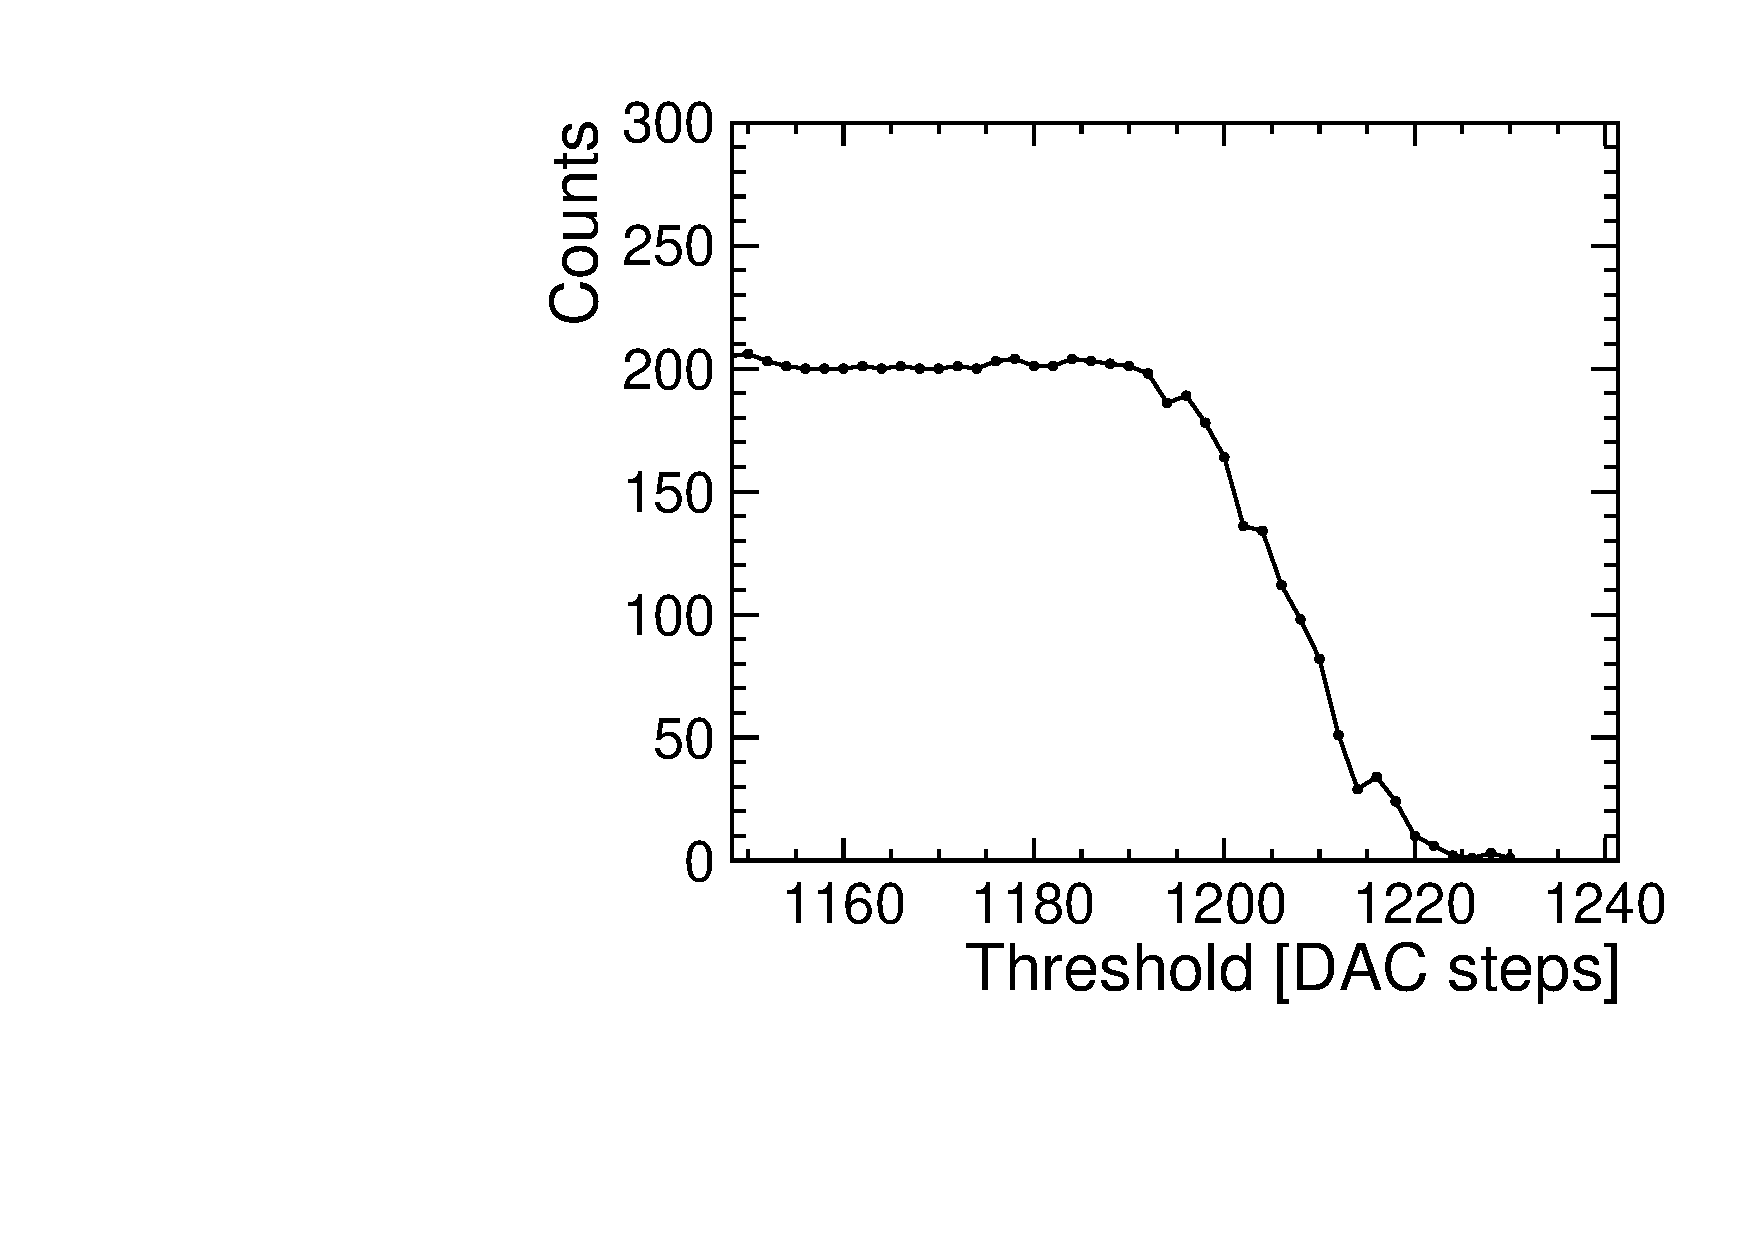
\includegraphics[width=\textwidth]{./figures/Calibration/W5_E2_scurve_ampl1.pdf}
    % \begin{tikzpicture} \node[anchor=south west,inner sep=0] (image)
    %   at
    %   (0,0){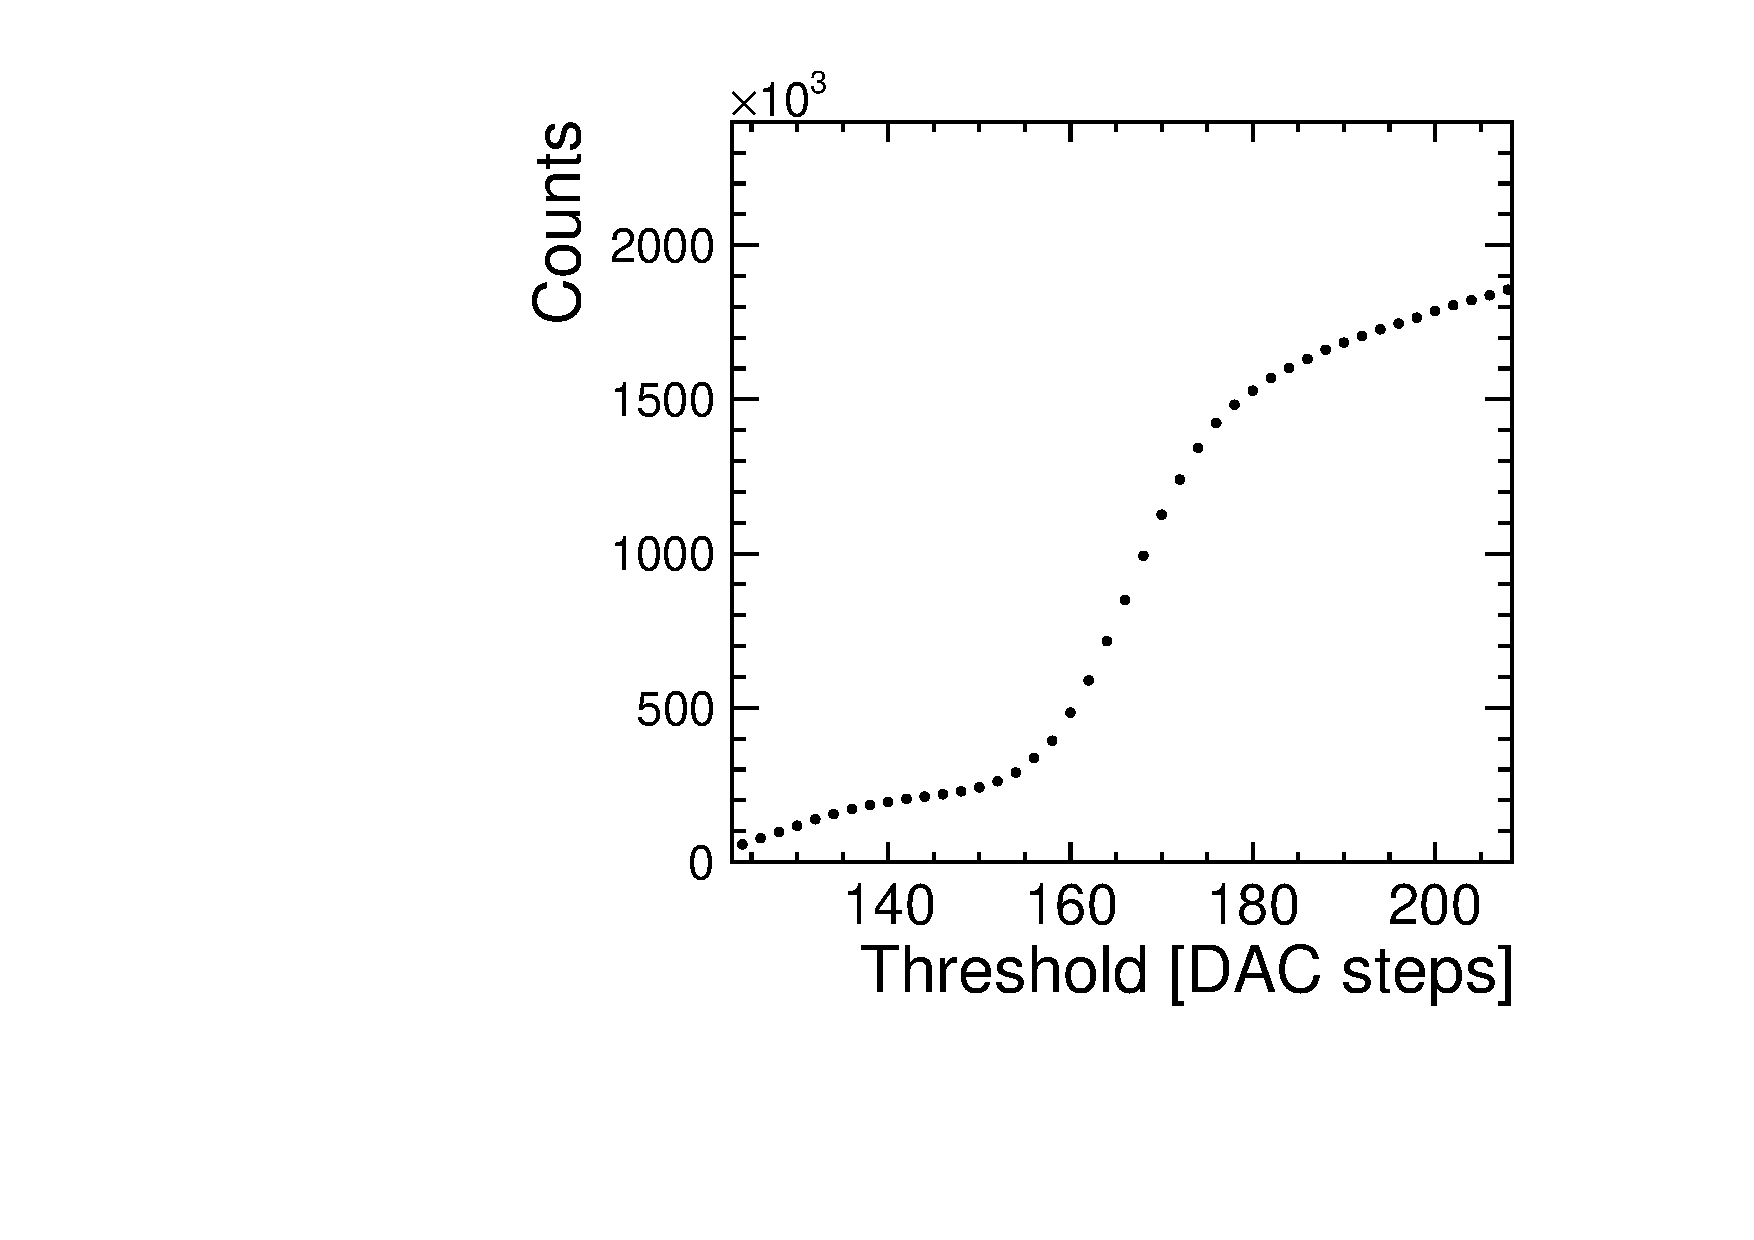
\includegraphics[width=\textwidth]{./figures/Calibration/L04-W0125_scurve_In.pdf}};
    %   % \draw[->,line width=.4pt, color=black](1.8, 1.4) -- (2.4, 1.4);
    %   \node[left, color=black] at (1.9, 1.6) {$K_{\beta}$}; %\draw[->,line
    %   width=.4pt, color=black](3, 2.7) -- (3.7, 2.7); \node[left,
    %   color=black] at (3.5, 2.7) {$K_{\alpha}$};
    % \end{tikzpicture}
    \caption{Measured S-curve}
    \label{fig:scurve_example}
  \end{subfigure} \hfill
  \begin{subfigure}[b]{0.45\textwidth}
    % 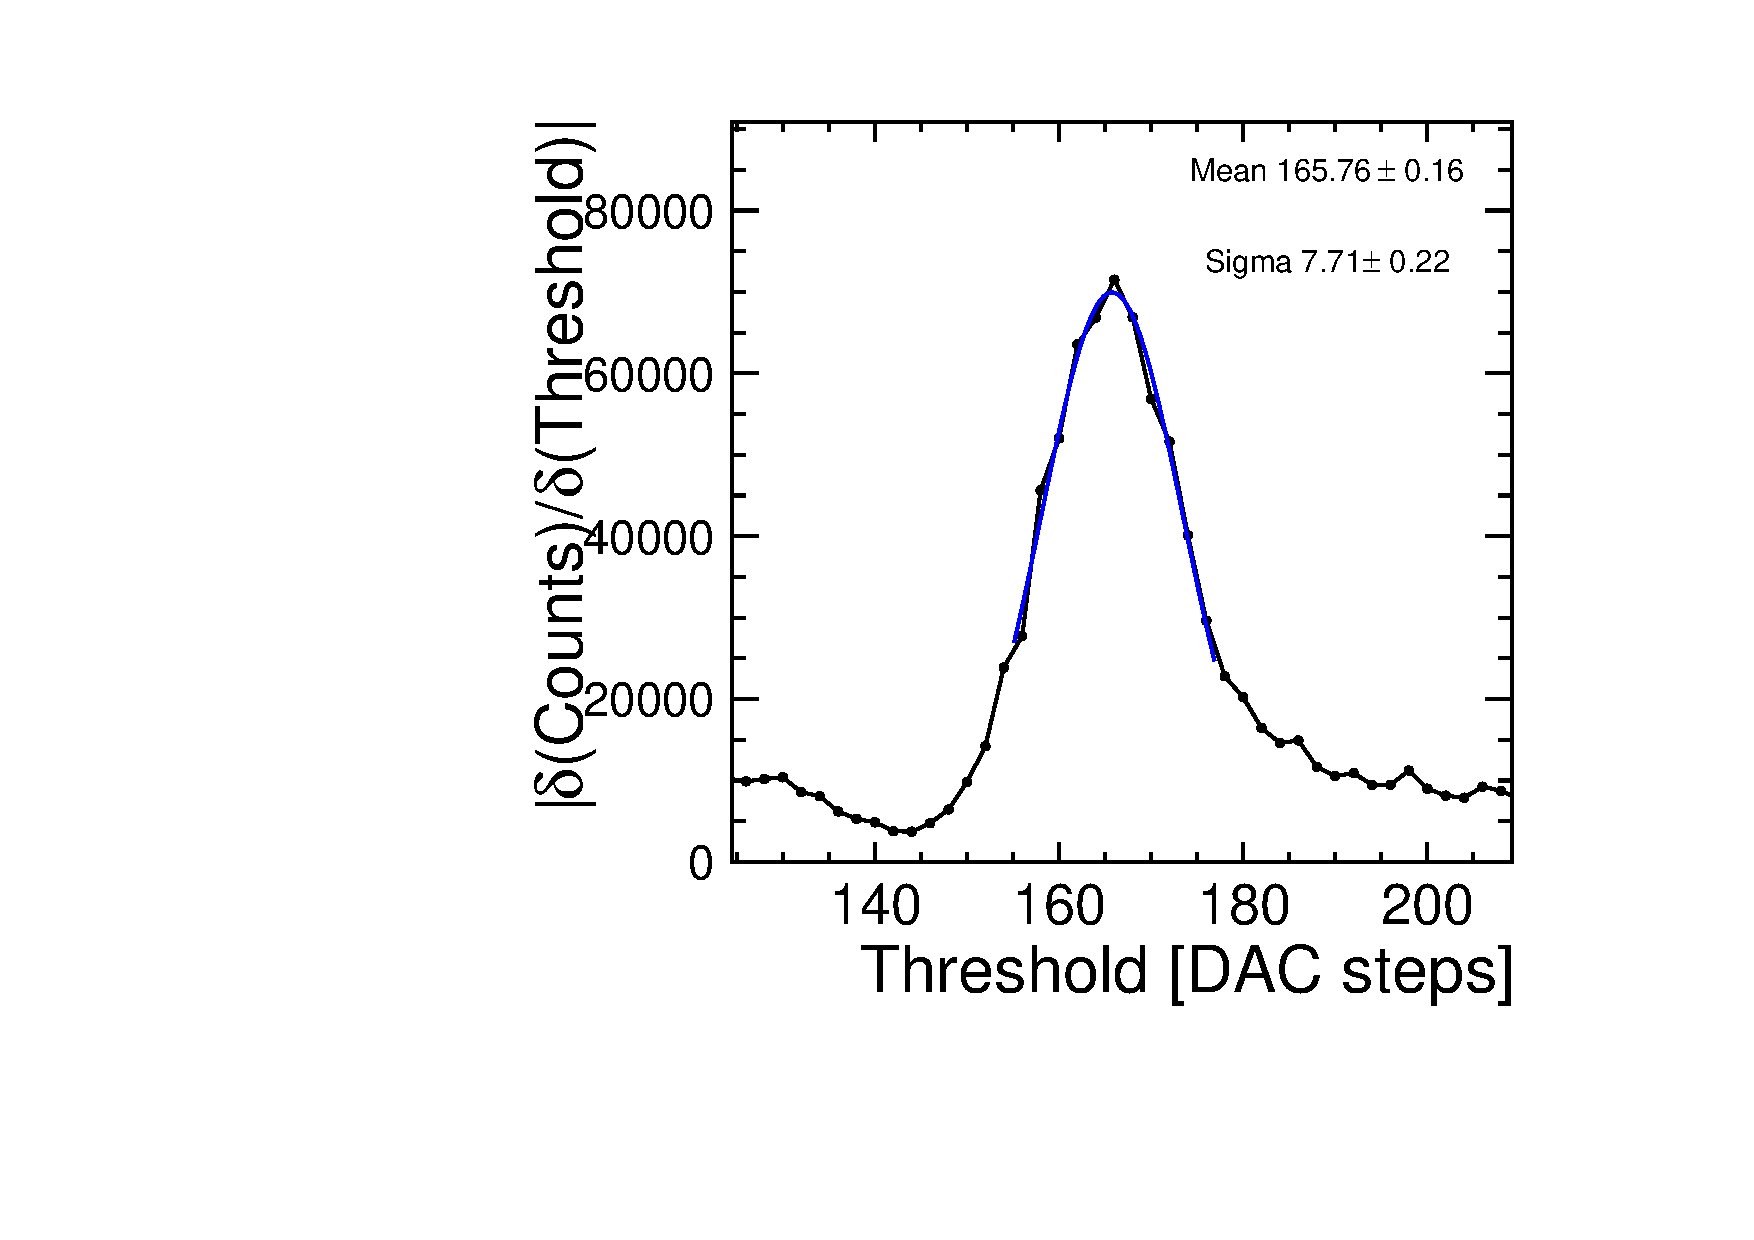
\includegraphics[width=\textwidth]{./figures/Calibration/L04-W0125_scurveDeriv_In.pdf}
    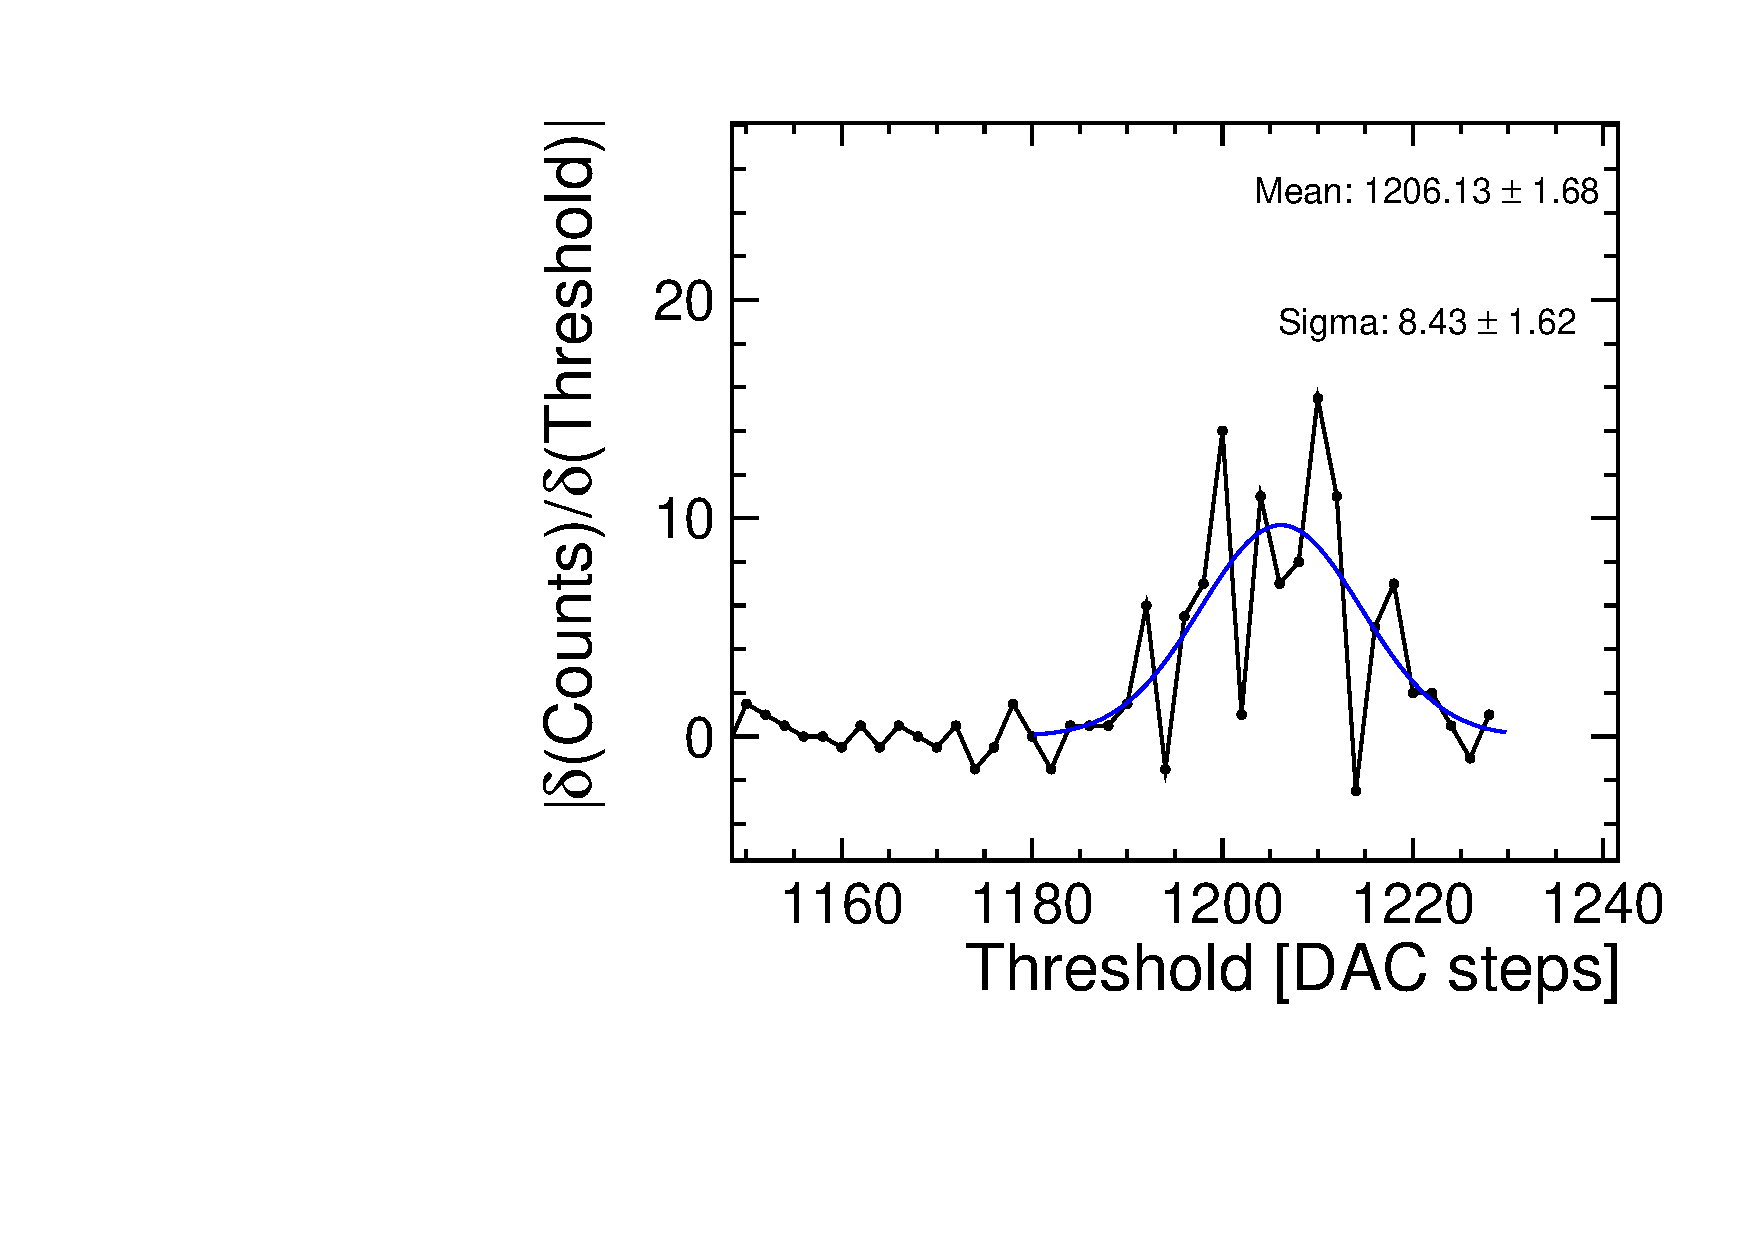
\includegraphics[width=\textwidth]{./figures/Calibration/W5_E2_deriv_scurve_ampl1.pdf}
    \caption{Derivative of the S-curve}
    \label{fig:deriv_example}
  \end{subfigure}
  \caption{(a) An example of a measured S-curve fitted with a sigmoid
    function and (b) the sigmoid's derivative fitted with a Gaussian
    function for the assembly W5\_E2 using a pulse height of 1000
    electrons for the pixel (0, 0) (see the coordinates system in
    \cref{fig:coordinateSystem}). This measurement is performed for
    all the pixels on the diagonal of the matrix for each assembly.}
  \label{fig:scurve_deriv_example}
\end{figure}

A linear fit is used to parametrise the relationship between the pulse
height and the threshold DAC given by the mean of the derivative of
the S-curves:
\begin{equation}
  THL_{DAC}=p \; THL_{e-} + q \; ,
  \label{eq:THLDAC}
\end{equation}
where $THL_{DAC}$ is the threshold DAC setting and $THL_{e-}$ the
corresponding energy (in number of electrons). 

\cref{fig:THLcalib_55-GNDGR-100} shows an example of the threshold
calibration obtained for the assembly W5\_E2 (see
\cref{sec:appendixFE_electronics} for all the assemblies). Each point
used for the fit corresponds to the mean of the Gaussian fitted to the
derivative of the sigmoid function fitting the S-curve for all the
diagonal pixels combined. The RMS of the mean is used as the error on
the mean. The RMS represents the threshold dispersion from one pixel
to another and corresponds to $\sim40$ electrons.

\begin{figure}[htbp]
  \centering
  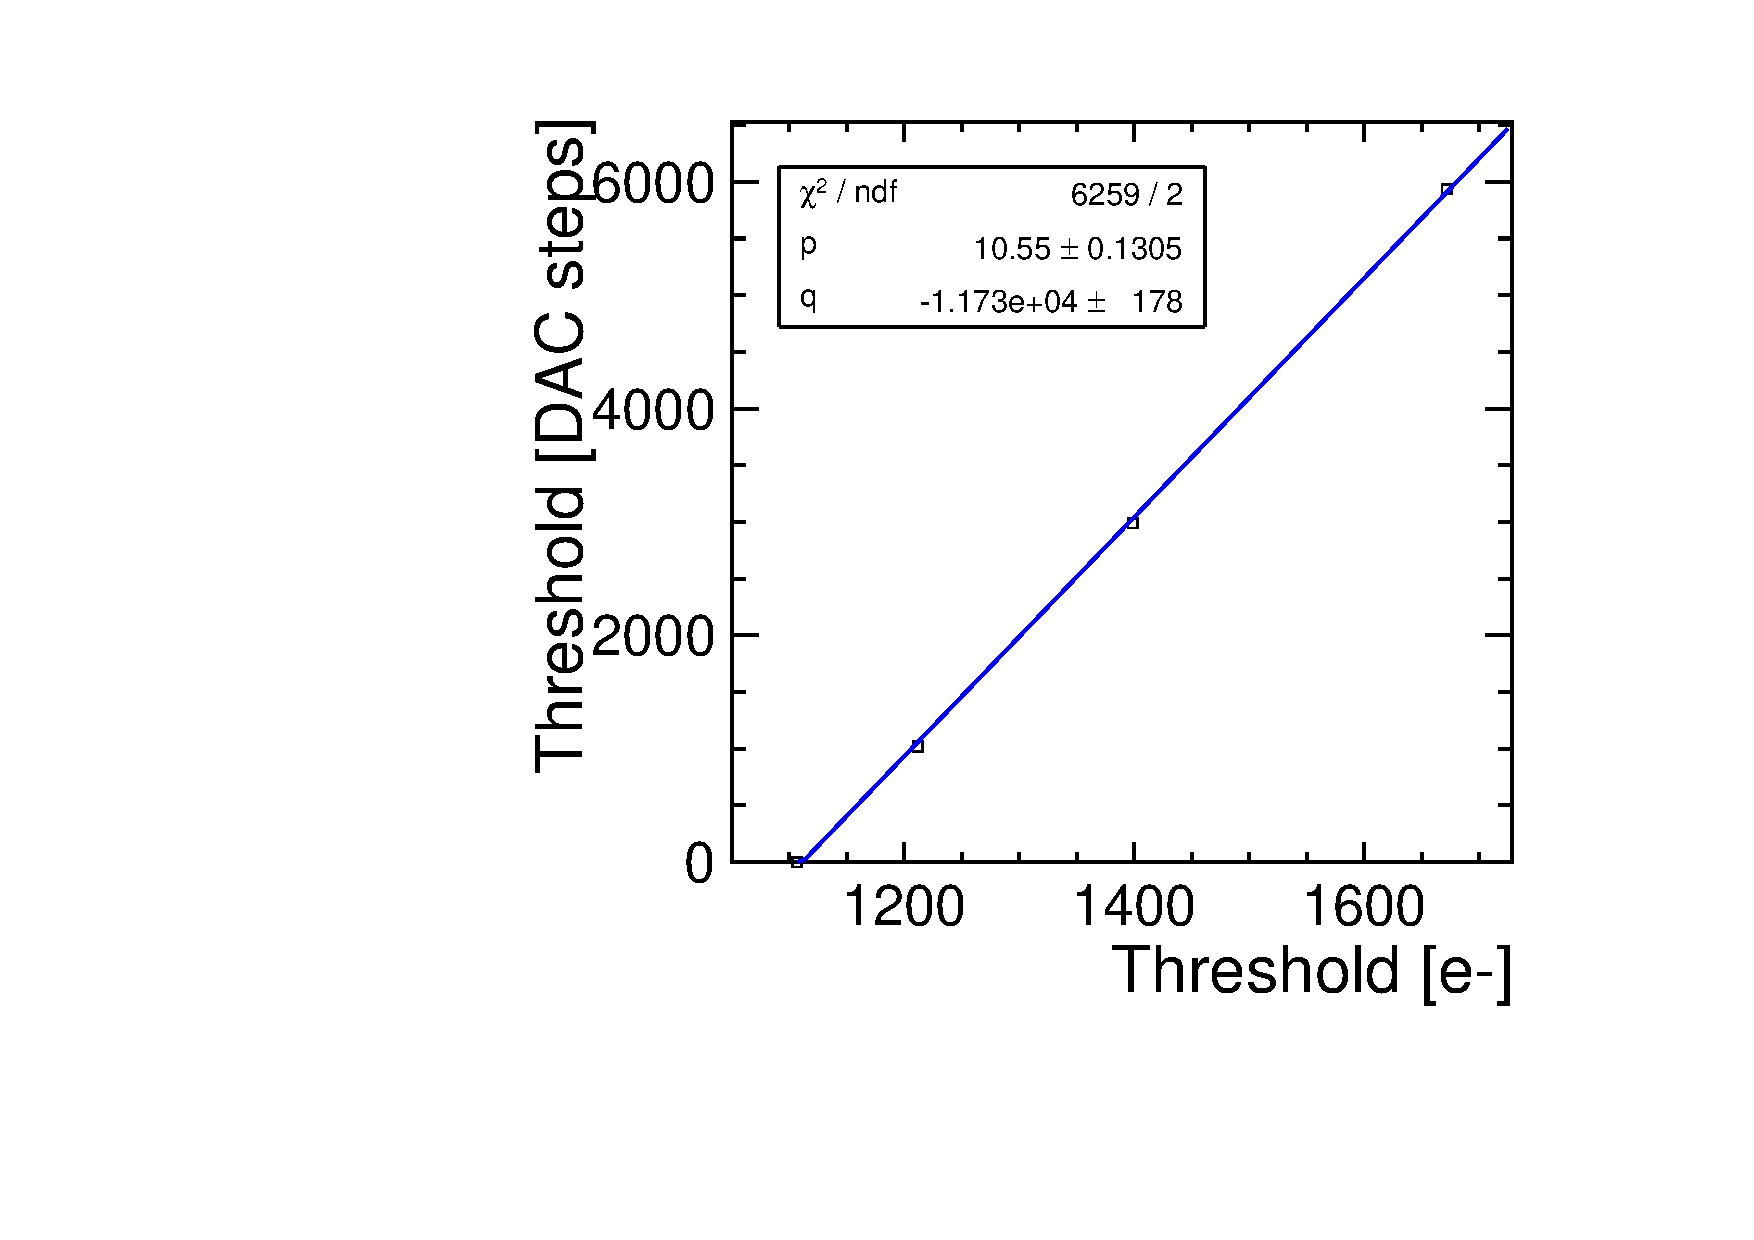
\includegraphics[width=0.5\textwidth]{./figures/Calibration/THLcalibration_W0005_E02.pdf}
  \caption{Threshold calibration for W5\_E2. Each point corresponds to
    the maximum gradient of the S-curve for each pulse height. A
    linear function as described in \cref{eq:THLDAC} was used to fit
    the data points and obtain the parameters $p$ and $q$.}
  \label{fig:THLcalib_55-GNDGR-100}
\end{figure}

% \begin{figure}[htbp]
%   \centering
%   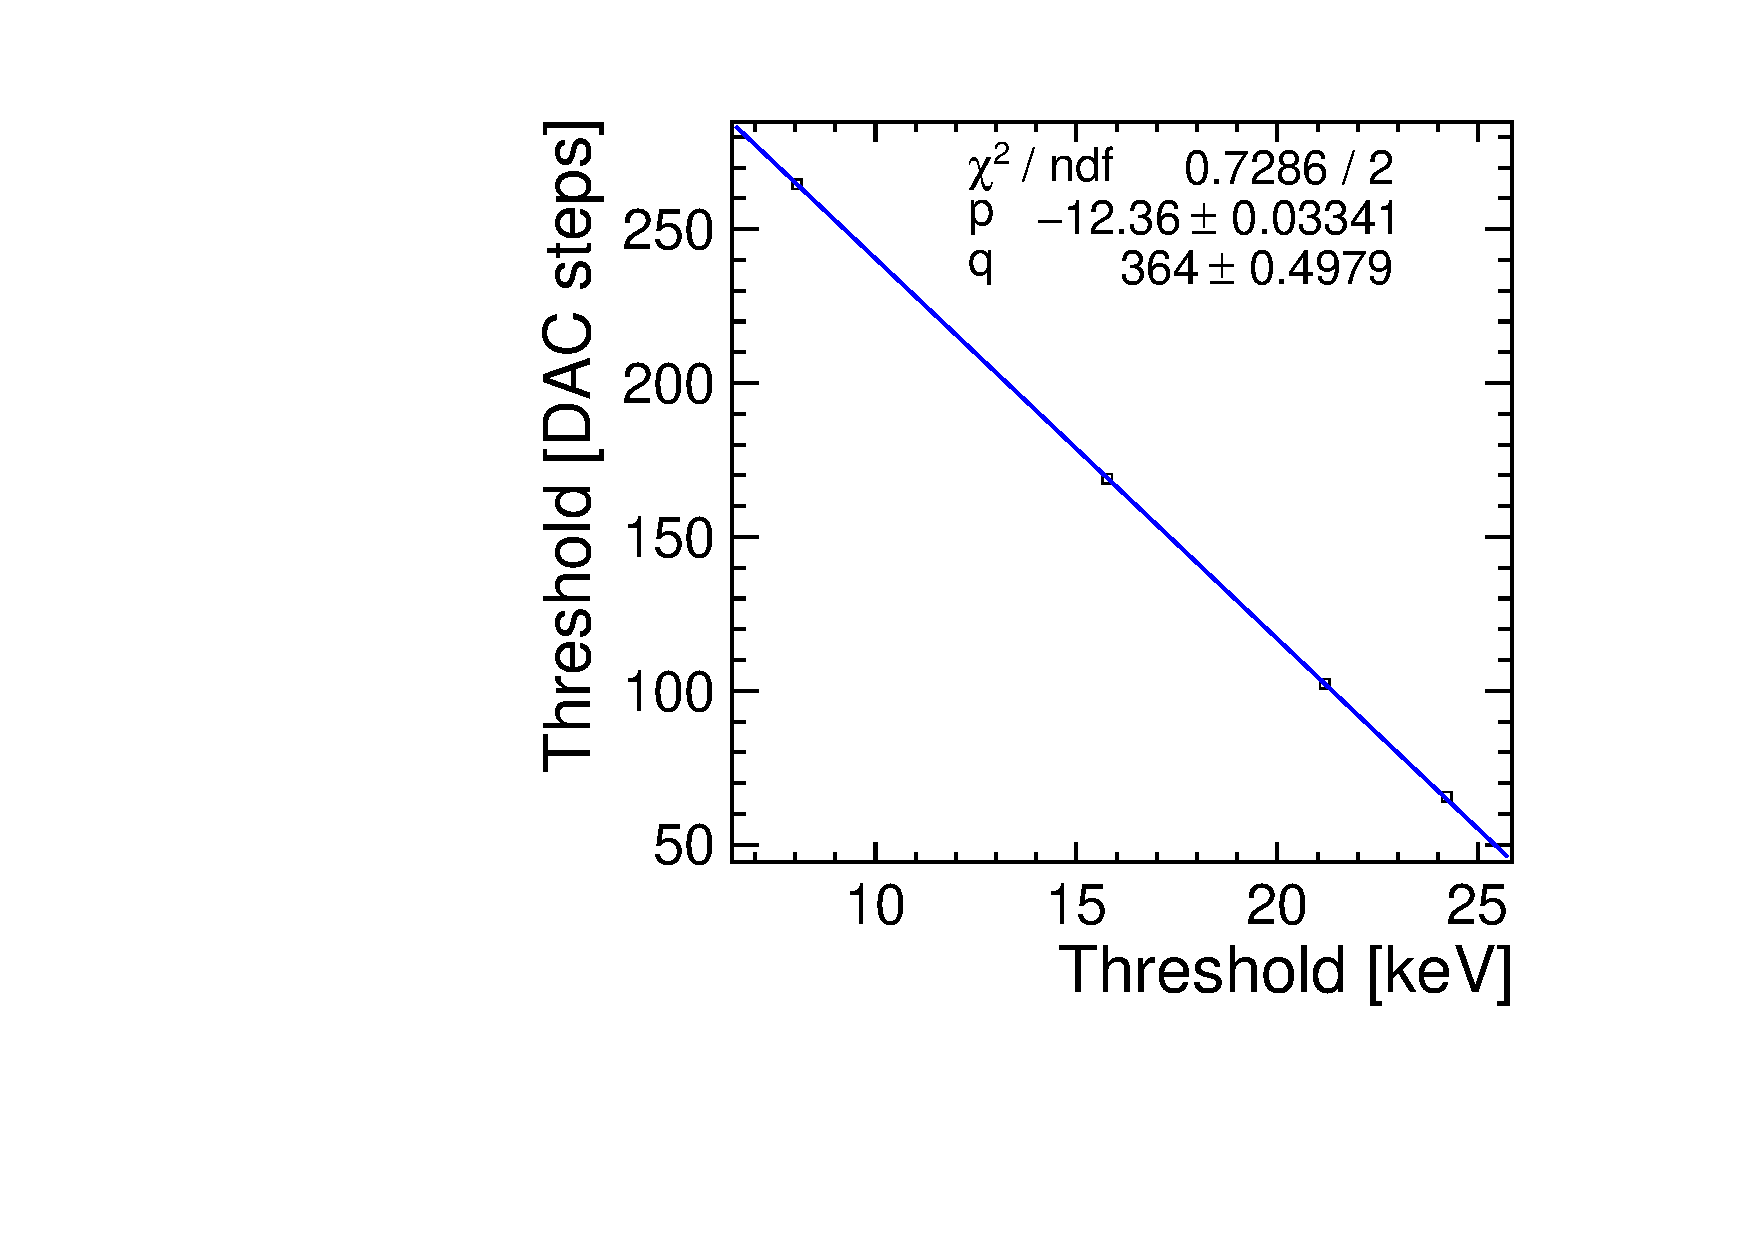
\includegraphics[width=0.5\textwidth]{./figures/Calibration/A06-W0110_THLcalibration.pdf}
%   \caption{Threshold calibration for A06-W0110. Each point corresponds
%     to the maximum gradient of the S-curve for each target (Cu, Zr, Pd
%     and In). A linear function as described in \cref{eq:THLDAC} was
%     used to fit the data points and obtain the parameters $p$ and
%     $q$.}
%   \label{fig:THLcalib_A06}
% \end{figure}

The operating threshold DAC for each assembly was converted to an
energy by solving \cref{eq:THLDAC} for $THL_{e-}$ with
$THL_{DAC}=THL_{DAC}^{op}$. The error on the evaluated threshold in energy
($THL_{e-}^{op}$) is obtained by the propagation of errors for the
inverse of \cref{eq:THLDAC}:
\begin{equation}
  \sigma_{THL_{e-}}^2(THL_{DAC})={{{(THL_{DAC}-q)^2} \over {p^4}} \sigma_{p}^2} +
        {\frac{1}{p^2} \sigma_{q}^2}+
        {2 {{THL_{DAC}-q} \over p^3} \sigma_{pq}^2} \; ,
        \label{eq:THLerror}
\end{equation}
where $p$, $q$ are given by the linear fit using \cref{eq:THLDAC} with
standard deviations $\sigma_{p}$, $\sigma_{q}$ and covariance
$\sigma_{pq}$.

\cref{tab:THLcalibration} summarises the fit parameters p and q, the
operating threshold DAC and its conversion into energy deposition in
number of electrons for all the assemblies listed in
\cref{tab:THLcalibration}.

\begin{table}[htbp]
  \centering
  \caption{Threshold fit parameters p and q, the operating threshold
    DAC and its conversion into energy deposition.}
  \label{tab:THLcalibration}
  \begin{tabular}{lcccc}
    \toprule
    Assembly & p [DAC steps/ke\textsuperscript{-}] & q [DAC steps] & THL\textsubscript{DAC}\textsuperscript{op} [DAC steps] & THL\textsubscript{e-}\textsuperscript{op} [e\textsuperscript{-}] \\
    \midrule
    W19\_G7 & $87.4\pm1.4$ & $1145.9\pm2.9$ & 1190 & $505\pm31$ \\
    W19\_F7 & $92.0\pm1.5$ & $1134.9\pm3.4$ & 1187 & $566\pm33$ \\
    W19\_L8 & $89.9\pm1.5$ & $1083.9\pm3.1$ & 1133 & $546\pm31$ \\
    W19\_C7 & $90.4\pm1.4$ & $1096.4\pm3.5$ & 1148 & $571\pm34$ \\
    W5\_E2  & $94.5\pm1.6$ & $1109.3\pm3.5$ & 1160 & $537\pm33$ \\
    W5\_F1  & $89.0\pm1.3$ & $1105.3\pm3.1$ & 1153 & $536\pm31$ \\
    \bottomrule
  \end{tabular}
\end{table}



For further verification of these results, the Timepix3 DAC step gain
for each assembly is calculated to be around
$\pm11$~e\textsuperscript{-}/step, in agreement
with~\cite{Timepix3Poikela}.

The mean of the Gaussian distribution with no input test-pulse
injection defines the baseline of the chip and its width the
electronic noise. The error on the mean corresponds to the threshold
dispersion across the full matrix. For all assemblies the noise varies
between 6 to 7 DAC values which corresponds to 70 to 80 electrons and
in agreement with~\cite{art:tmpx}. The error on the noise is obtained
by the error propagation of
\cref{eq:THLDAC}. \cref{tab:THLcalibration_noise} summarises the
baseline mean, the threshold DAC step, the electronic noise and its
conversion into energy deposition for the assemblies listed in
\cref{tab:THLcalibration}.


%%%%%%%%%%%%%%%%%%%%%%%%%%%%%%%%%%%%%%%%%%%%%%%%%%

\begin{table}[htbp]
  \centering
  \caption{Measured baseline mean, threshold DAC step gain, the electronic noise
    and its conversion into energy deposition.}
  \label{tab:THLcalibration_noise}
  \resizebox{\textwidth}{!}{\begin{tabular}{lcccc}
    \toprule
    Assembly & Baseline mean [DAC steps] & Threshold DAC step [e\textsuperscript{-}] & Noise [DAC steps] & Noise [e\textsuperscript{-}] \\
    \midrule
    W19\_G7 & $1143.9\pm3.2$ & $11.4\pm0.2$ & $6.9\pm0.9$ & $78.5\pm10.3$ \\
    W19\_F7 & $1131.7\pm3.8$ & $10.9\pm0.2$ & $7.1\pm0.9$ & $76.7\pm9.9$ \\
    W19\_L8 & $1082.0\pm3.3$ & $11.1\pm0.2$ & $7.0\pm0.9$ & $77.9\pm10.2$ \\
    W19\_C7 & $1092.8\pm3.9$ & $11.1\pm0.2$ & $7.4\pm1.1$ & $82.0\pm12.4$ \\
    W5\_E2  & $1106.9\pm3.9$ & $10.6\pm0.2$ & $7.2\pm1.1$ & $75.7\pm11.8$ \\
    W5\_F1  & $1103.6\pm3.4$ & $11.2\pm0.2$ & $6.7\pm0.9$ & $75.4\pm9.7$ \\
%    W2\_J5  & $1231.70\pm0.034$ & $-9.177\pm0.000$ & $11.826\pm0.041$ & $108.53\pm0.379$ \\
    \bottomrule
  \end{tabular}}
\end{table}

%% --------------------------------------------- %%
\subsection{TOT-energy calibration}
\label{sec:EnergyCalibration}

The TOT calibration parametrises the relationship between the energy
deposited and the TOT measurement. Due to the non-linearity of the
Timepix3 charge preamplifier, this relationship is modeled as a
hyperbola. The function used to fit the data points is called a
\textit{surrogate function} and is obtained as:

\begin{equation}
  \text{TOT} = a \, E + b - \frac{c}{E - t} \; ,
  \label{eq:TOTsurrogateFunction}
\end{equation}

where TOT denotes Time-Over-Threshold, $E$ the deposited energy and
$a, b, c, t$ are the parameters to be found~\cite{Jakubek2008155}. The
inverse of the surrogate function is defined as:

\begin{equation}
  E = { {t \cdot a - \text{TOT} -b + \sqrt{\left(b+t \cdot a -\text{TOT}\right)^2+4\cdot a \cdot c}} \over {2a} } \; .
  \label{eq:inverseTOTsurrogateFunction}
\end{equation}

In \cref{eq:TOTsurrogateFunction}, for higher values of the energy,
the relationship between TOT and $E$ is linear with gradient $a$ and
intercept $b$ since the term $aE+b$ dominates. At low energy, the term
$c/(E-t)$ becomes important. The parameter $c$ defines the amount of
curvature in the function. An asymptote occurs at $E=t$. The point at
which the fit crosses the x-axis (TOT=0) corresponds to the threshold:
below the threshold no charge can be detected. The calibrated
threshold is used as a data point for the surrogate fit at the
crossing-point on the $x$-axis. The range for the TOT and the boundary
between low energy (non-linear response) and high energy (linear
response) depend on the clock frequency, the threshold and the
I\textsubscript{krum} value.

For the calibration of the assemblies, the Timepix3 ASICs are operated
in TOT mode and the test-pulse injection is used
(\cref{eq:testpulseCharge}). Test pulses with heights ranging from
$0\,\mv$ to $800\,\mv$ (corresponding to 0 electrons to 16000
electrons) are sent to each pixel. For each pulse height, 100
test-pulses are sent. The sum of the TOTs and also the sum of the
square of the TOTs for each pulse height is recorded. The mean of the
TOT response and the standard deviations are then calculated. Finally,
the data are fitted with the surrogate function as given in
\cref{eq:TOTsurrogateFunction} for each pixel, to determine the
pixel-by-pixel energy calibration of the assembly.

\cref{tab:timepix3Operation} summarises the DAC settings used for the
operation of the Timepix3 assemblies in test beams. The same settings
are as well used for the calibration. \cref{fig:TOTcalib_55GNDGR100}
shows the pixel-by-pixel calibration for assembly W5\_E2 operated at
two different threshold DACs of 1160 (537 electrons) and 1190 (855
electrons). For a higher threshold, the curves are shifted towards
higher energy values on the x-axis but the slope (parameter $a$)
remains the same.

\begin{table}[htbp]
  \centering
  \caption{DAC settings for the operation and calibration of the
    Timepix3 assemblies. VFBK is a programmable DAC to determine the
    baseline voltage of the chip.}
  \label{tab:timepix3Operation}
  \begin{tabular}{ c c c c }
    \toprule
    I\textsubscript{krum} & TOT/TOA Clock & FTOA Clock & VFBK \\
    \midrule
    10 & $40\,\megahertz$ & $640\,\megahertz$ & 150 \\
    \bottomrule
  \end{tabular}
\end{table}

\begin{figure}[htbp] \centering
  \begin{subfigure}[b]{0.45\textwidth}
    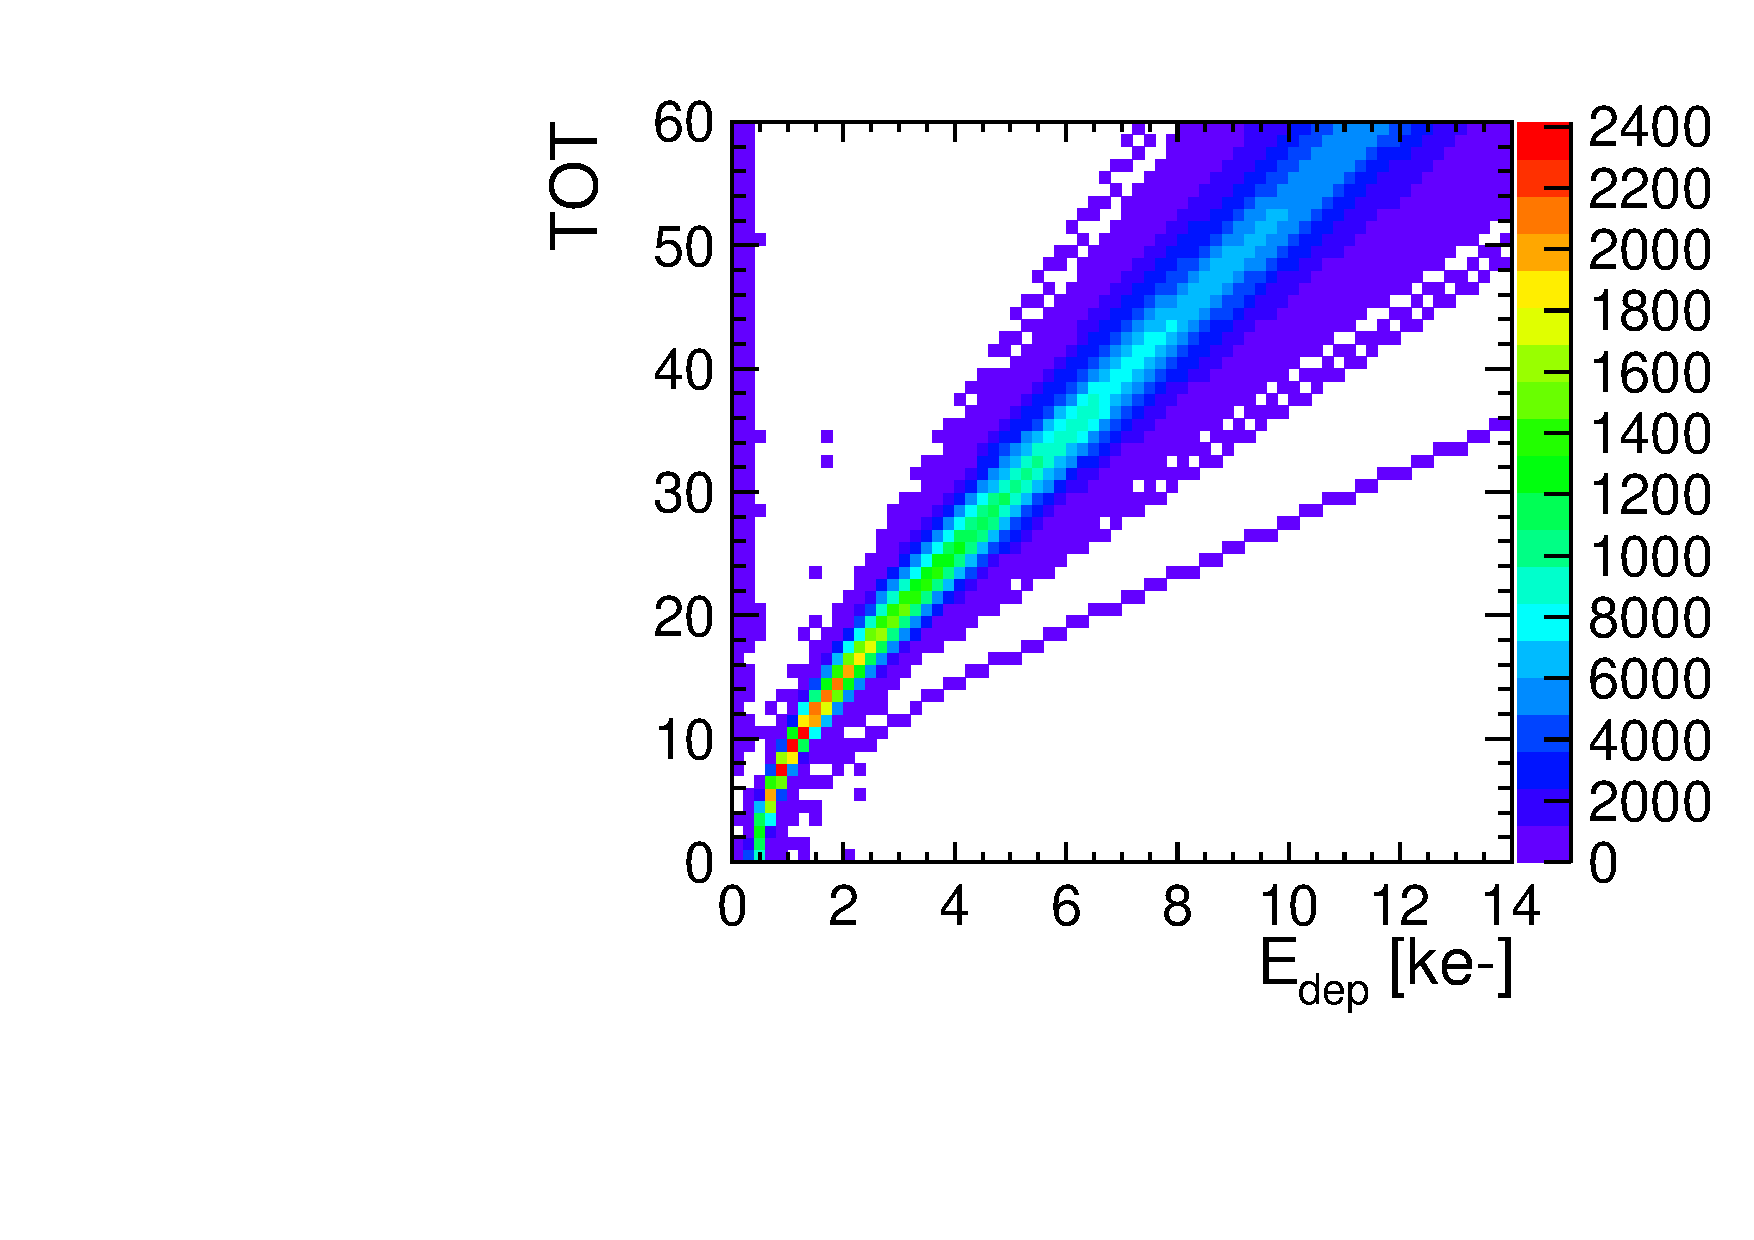
\includegraphics[width=\textwidth]{./figures/Calibration/TOTcalibration_W0005_E02_thresh1160.pdf}
    \caption{}
  \end{subfigure} \hfill
  \begin{subfigure}[b]{0.45\textwidth}
    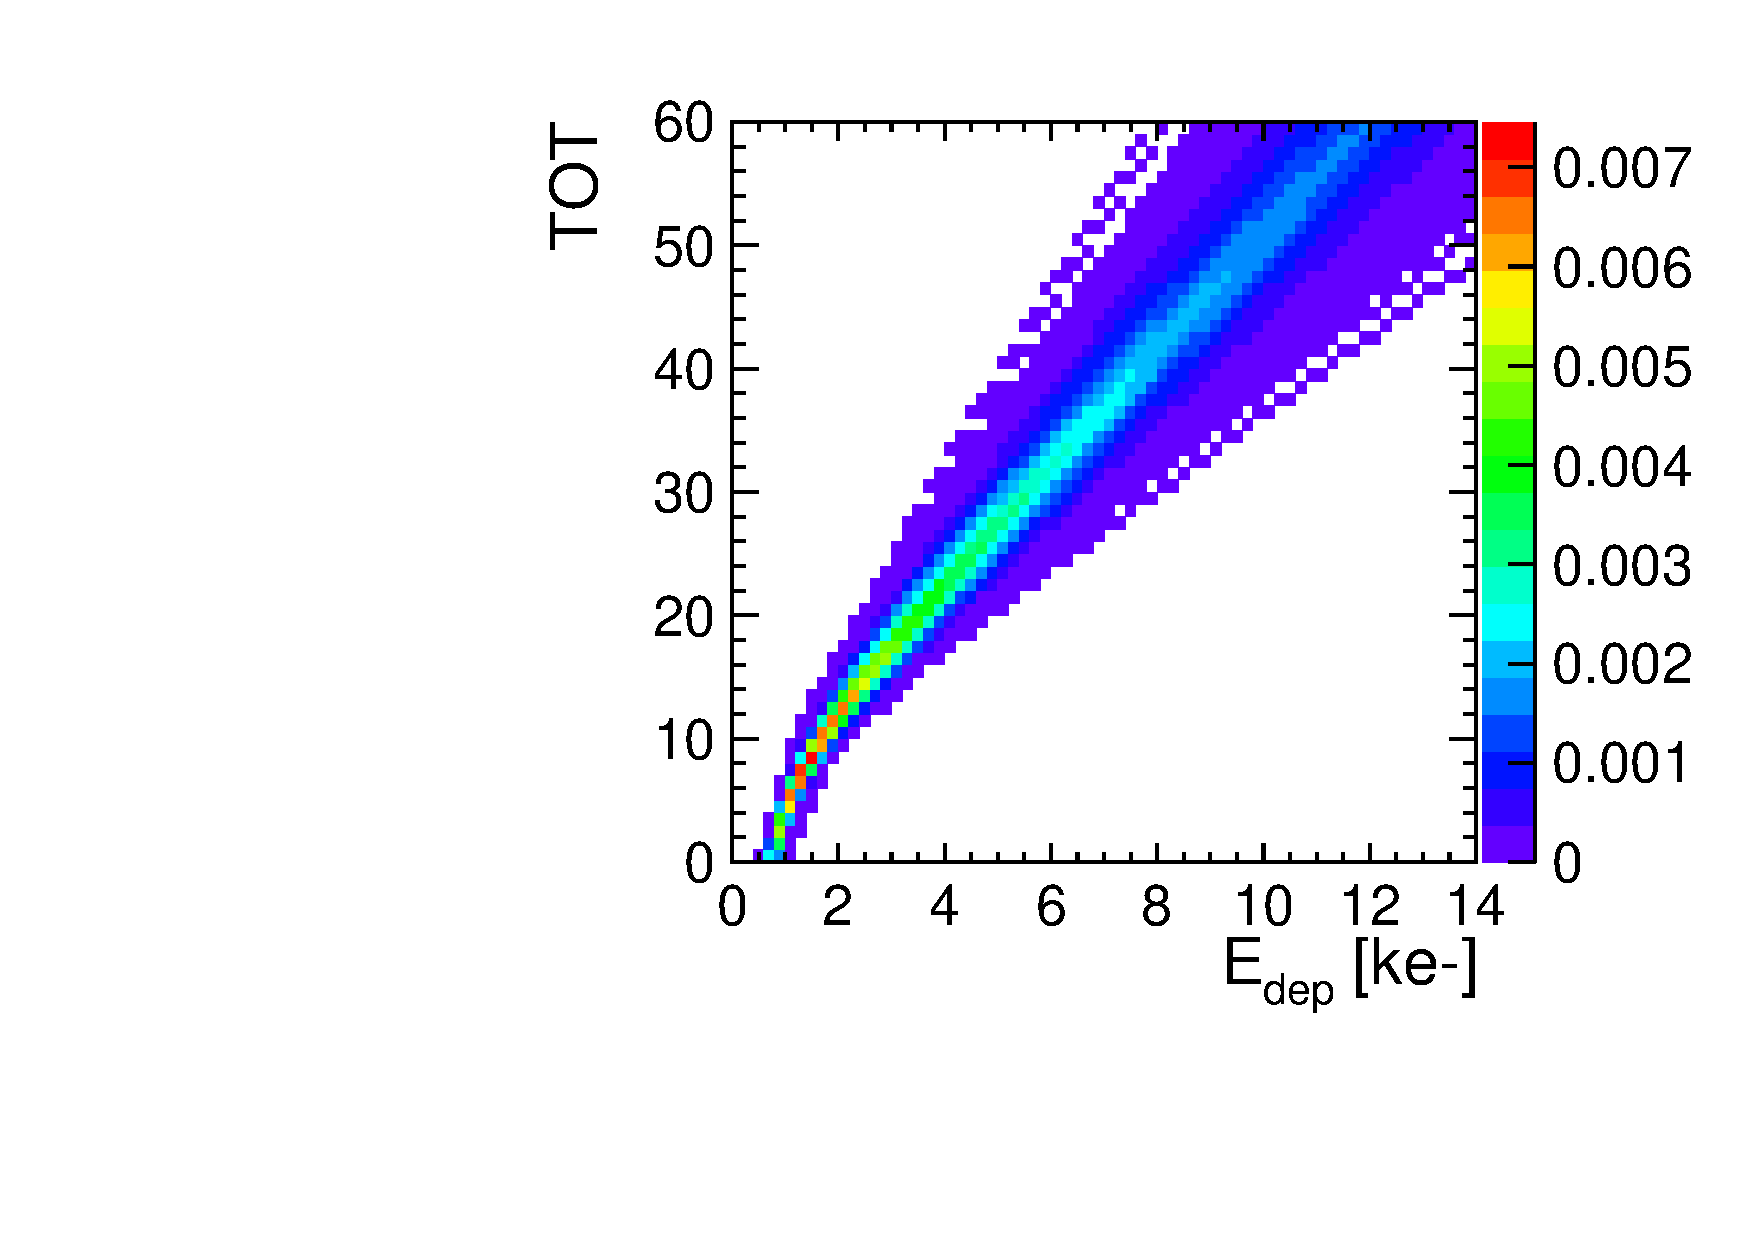
\includegraphics[width=\textwidth]{./figures/Calibration/TOTcalibration_W0005_E02_thresh1190.pdf}
    \caption{}
  \end{subfigure}
  \caption{Pixel-by-pixel calibration of the TOT for assembly W5\_E2
    operated at the threshold DACs of (a) THL=1160 (561 electrons) and
    (b) THL=1190 (878 electrons).}
  \label{fig:TOTcalib_55GNDGR100}
\end{figure}

%% The calibration results for the other assemblies are shown in
%% \cref{sec:appendixFE_electronics}.


\section{Summary}
\label{sec:Summary_calibration}

This chapter gives an overview on the Timepix3 readout ASIC which is
used in the tracking planes of the CLICdp Timepix3 telescope (see
\cref{ch:Telescope}) and also employed as a test vehicle for the
characterisation of thin sensors (see \cref{ch:ThinSensorsStudies})
and active-edge sensors (see \cref{ch:ActiveEdgeSensors}).

The test-pulse injection method is used to calibrate the operating
threshold and the TOT value into energy depositions. In
\cref{ch:ThinSensorsStudies}, the calibration is applied to the
test-beam data and validated with simulations.

%%%%%%%%%%%%%%%%%%%%%%%%%%%%%%%%%%%%%%%%%%%%%%%%%%%%%%%%
%%%%%%%%%%%%%%%%%%%%%%%%%%%%%%%%%%%%%%%%%%%%%%%%%%%%%%%%
%%%%%%%%%%%%%%%%%%%%%%%%%%%%%%%%%%%%%%%%%%%%%%%%%%%%%%%%
% \begin{table}[htbp]
%   \caption{Measured DAC step gain.}
%   \label{tab:DACStep}
%   \centering
%   \begin{tabular}{ c c c }
%     \toprule
%     Assembly & Threshold DAC step [\ev] & Threshold DAC step [\Pem] \\
%     \midrule
%     A06-W0110  & $81\pm0.009$ & $22.475\pm0.025$  \\
%     C04-W0110  & $85\pm0.039$ & $23.544\pm0.011$ \\
%     L04-W0125 &  $86\pm0.022$ & $23.775\pm0.006$ \\
%     B06-W0125  & $86\pm0.120$ & $23.978\pm0.033$ \\
%     \bottomrule
%   \end{tabular}
% \end{table}

% Threshold measurements were not completed for assemblies B07-W0125 and
% D09-W0126. Assembly B07-W0125 did not fully deplete due to a broken
% corner of the sensor. The derivative of the CuXRF S-curve did not form
% a peak as the photon energy was close to the noise level. Assembly
% D09-W0126 was not operating as expected for a $100\,\micron$
% sensor. Therefore the calibration of these assemblies was done without
% threshold measurements.



%% \begin{table}[htbp]
%%   \centering
%%   \caption{Advacam active-edge n-in-p planar pixel sensor assemblies. The edge distance is defined by the distance between the last pixel implant and the physical sensor edge.}
%%   \label{tab:NominalThreshold}
%%   \resizebox{\textwidth}{!}{\begin{tabular}{lccc}
%%       \toprule
%%       Assembly & Nominal THL\textsubscript{DAC}\textsuperscript{op} [DAC steps] & Nominal THL\textsubscript{e-}\textsuperscript{op} [electrons]\\
%%       \midrule
%%       20-NGR & 1190 & 466.5\\
%%       23-FGR & 1187 & 532.4\\ \hline
%%       28-GNDGR & 1133 & 517.8\\
%%       55-GNDGR & 1148 & 553.7\\
%%       55-GNDGR-100 & 1160 & 537.9\\ \hline
%%       55-GNDGR-150 & 1153 & 441.2\\
%%       \bottomrule
%%   \end{tabular}}
%% \end{table}


% \begin{table}[htbp]
%   \caption{Threshold fit parameters $p$ and $q$, the operating
%     threshold DAC and its conversion into energy.}
%   \label{tab:evalTHL} 
%   \centering
%   \begin{tabular}{ c c c c c }
%     \toprule
%     Assembly & $p$ [DAC steps/\kev] & $q$ [DAC steps] & $THL_{DAC}^{op}$ [DAC steps] & $THL_{\kev}^{op}$ [\kev] \\
%     \midrule
%     A06-W0110 & $-12.36\pm0.03$ & $364.0\pm0.50$ & 326 & $3.077\pm0.033$ \\
%     C04-W0110 & $-11.8\pm0.02$ & $441.6\pm0.42$ & 405 & $3.102\pm0.030$ \\
%     L04-W0125 & $-11.68\pm0.02$ & $448.6\pm0.31$ & 410 & $3.303\pm0.023$ \\
%     B06-W0125 & $11.58\pm0.037$ & $390.6\pm0.80$ & 435 & $3.836\pm0.057$ \\
%     \bottomrule
%   \end{tabular}
% \end{table}



% \begin{figure}[htbp]
%   \centering
%   \begin{tikzpicture}
%     \begin{scope}[x={(image.south east)},y={(image.north west)}]
%       % pulse
%       \draw[-, thick] (0.1, 0.8) -- (0.2, 0.8);
%       \draw[-, thick] (0.2, 0.8) -- (0.21, 0.98);
%       \draw[-, thick] (0.21, 0.98) -- (0.22, 0.8);
%       \draw[-, thick] (0.22, 0.8) -- (1, 0.8);

%       % shaper
%       \draw[-, thick] (0.1, 0.5) -- (0.2, 0.5);
%       \draw[-, thick] (0.2, 0.5) -- (0.22, 0.7);
%       \draw[-, thick] (0.22, 0.7) -- (0.8, 0.5);
%       \draw[-, thick, dashed, green] (0.1, 0.55) -- (0.8, 0.55);
%       \draw[-, thick] (0.8, 0.5) -- (1, 0.5);

%       % comparator
%       \draw[-, thick] (0.1, 0.3) -- (0.21, 0.3);
%       \draw[-, thick] (0.21, 0.3) -- (0.21, 0.4);
%       \draw[-, thick] (0.21, 0.4) -- (0.65, 0.4);
%       \draw[-, thick] (0.65, 0.4) -- (0.65, 0.3);
%       \draw[-, thick] (0.65, 0.3) -- (1, 0.3);

%       \timing [] at (0.11, 0.2) {HLLHHLLHHLLHHLLHHLLHHLLHH};
%       \draw[arrows=<->, thick](0.21, 0.15)--(0.65, 0.15) node [pos=0.5, below]
%       {\textbf{TOT (3 counts)}};

%       \timing [] at (0.1,0.0) {llllllhlhlhlhllllllllllllllllllllllllllllllllllllll};

%       \draw[-, thick, dashed, blue] (0.21, 0.55) -- (0.21, 0.0);
%       \draw[-, thick, dashed, blue] (0.65, 0.55) -- (0.65, 0.0);

%       \draw[-, thick, dashed, red] (0.355, 0.2) -- (0.355, 0.0);

%       \draw[arrows=<->, thick](0.21, -0.05)--(0.35, -0.05) node [pos=0.5, below]
%       {\textbf{FTOA (4 counts)}};


%       \node[left] at (0.1, 0.8) {Sensor pulse};
%       \node[left, green] at (0.1, 0.6) {Threshold};
%       \node[left] at (0.1, 0.5) {Pulse after shaping};
%       \node[left] at (0.1, 0.3) {Discriminator output};
%       \node[left] at (0.1, 0.2) {General clock}; %$40\,\megahertz$ Clk}
%       \node[left] at (0.1, 0.0) {FTOA clock}; %$640\,\megahertz$ Clk (FTOA)     


%     \end{scope}
%   \end{tikzpicture}
%   \caption{Schematic overview of the Time-over-Threshold (TOT) and
%     Time-of-Arrival (TOA) measurements for the Timepix3 readout chips.}
%   \label{fig:TOT_TOA_concept}
% \end{figure}
